\section{Proofs}\label{app:proofs}

Throughout, $F_k=N_k^{-1}\sum_{i=1}^{N_k}\delta_{S_{k,i}}$ is the score distribution of family $k$ (for the test family it involves unobserved labels and is used only in the analysis), and $\gamma_{K+1}(C)=F_{K+1}((-\infty,\hat q])$ because a test variant is covered iff its score is at most $\hat q$.

\paragraph{Comparison step for~\eqref{eq:threshold}.}
Fix weights $p_1,\dots,p_{K+1}$ and define the oracle measure $\mu=\sum_{k=1}^{K+1}p_kF_k$ and $q=\Qt_{1-\alpha}(\mu)$. The computable $\hat\mu$ moves the mass $p_{K+1}$ from $F_{K+1}$ to $+\infty$, so $\hat\mu((-\infty,u])\le\mu((-\infty,u])$ for every $u$, hence $\hat q\ge q$ and $\gamma_{K+1}(C)\ge F_{K+1}((-\infty,q])$. Also $\mu((-\infty,q])\ge1-\alpha$ by right-continuity.

\begin{proof}[Proposition~\ref{prop:hcp}]
With $\omega\equiv1$, $p_k=1/(K+1)$ and $q$ is a symmetric function of $(G_1,\dots,G_{K+1})$. By exchangeability, $\E[F_{K+1}((-\infty,q])]=\E[(K+1)^{-1}\sum_kF_k((-\infty,q])]=\E[\mu((-\infty,q])]\ge1-\alpha$, and the comparison step gives $\Cov(C)\ge1-\alpha$.
\end{proof}

\begin{proof}[Theorem~\ref{thm:conditional}]
Let $L^o(b)=\sum_{k=1}^{K+1}N_k^{-1}\sum_i\rho_\tau(S_{k,i}-\Phi(D_k)^\top b)$ be the oracle objective, in which the test family enters with its true scores. It is convex, piecewise linear and nonnegative, so its minimizers form a nonempty closed convex polyhedron; let $\tilde b$ be the one of minimum Euclidean norm (a measurable function of the data, for example as the limit of the ridge-penalized minimizers as the penalty vanishes; only its symmetry is used), $\tilde g=\Phi^\top\tilde b$, and $\tilde\gamma_k=N_k^{-1}\sum_i\1\{S_{k,i}\le\tilde g(D_k)\}$.

\emph{(a) First-order condition.} Let $f=\Phi^\top b_f$ with $f(D)\ge0$ $P$-a.s.; then $f(D_k)\ge0$ for every $k$ almost surely, which is all the argument uses. The right derivative of $t\mapsto\rho_\tau(S-\tilde g(D)-tf(D))$ at $t=0$ is $f(D)(\1\{S\le\tilde g(D)\}-\tau)$ (if $S=\tilde g(D)$, the residual is $-tf(D)\le0$ for $t>0$). The right derivative of $t\mapsto L^o(\tilde b+tb_f)$ at $0$ is therefore $\sum_{k=1}^{K+1}f(D_k)(\tilde\gamma_k-\tau)$, which is nonnegative at a minimizer.

\emph{(b) Symmetry.} $L^o$, and hence $\tilde b$, is invariant to permutations of the families, so the pairs $(f(D_k),\tilde\gamma_k)$, $k\le K+1$, are exchangeable under $P^{K+1}$ and $\E_{P^{K+1}}[f(D_{K+1})(\tilde\gamma_{K+1}-\tau)]=(K+1)^{-1}\E\sum_kf(D_k)(\tilde\gamma_k-\tau)\ge0$; the expectation exists because $\tilde\gamma\in[0,1]$ and $\E_Pf<\infty$.

\emph{(c) Change of measure.} For any bounded measurable $H$ of the families, $\E_{P^{K+1}}[f(D_{K+1})H]=\E_Pf(D)\cdot\E_{P^K\times Q_f}[H]$. With $H=\tilde\gamma_{K+1}-\tau$, (b) gives $\E_{P^K\times Q_f}[\tilde\gamma_{K+1}]\ge\tau$.

\emph{(d) The computable threshold dominates the oracle.} We show $\hat q\ge\tilde g(D_{K+1})$, which gives $\gamma_{K+1}(C)\ge\tilde\gamma_{K+1}$ and, with (c), the theorem. The argument follows Proposition~6 of~\cite{gibbs2025conformal} (imputing an upper bound $M$), with the supremum over the solution set in place of a min-norm solution, and $M\to\infty$. Write $\phi_t=\Phi(D_{K+1})$. If $L$ in~\eqref{eq:condcal} is unbounded below, $\hat q=+\infty$. Otherwise $A=\arg\min L$ is nonempty (a polyhedral function bounded below attains its minimum). Pick $M$ larger than every test score and than $\inf_{b\in A}\phi_t^\top b$, and let $L^M$ be $L^o$ with every test score replaced by $M$. Since $\rho_\tau(u)\ge\tau u$ with equality for $u\ge0$, $L^M(b)=L(b)+\tau\phi_t^\top b+\rho_\tau(M-\phi_t^\top b)\ge L(b)+\tau M$, with equality when $\phi_t^\top b\le M$, which holds for some $b\in A$; hence $\min L^M=\min L+\tau M$ and $\arg\min L^M\subseteq A$. Let $b'\in\arg\min L^M$, $a=\tilde g(D_{K+1})$ and $a'=\phi_t^\top b'$. Adding $L^o(\tilde b)\le L^o(b')$ and $L^M(b')\le L^M(\tilde b)$, the calibration terms cancel and $\sum_i[h_i(a)-h_i(a')]\le0$, where $h_i(c)=\rho_\tau(S_{K+1,i}-c)-\rho_\tau(M-c)$ is nondecreasing in $c$ because $S_{K+1,i}\le M$ and $\rho_\tau$ is convex. If $a'<a$, then $h_i(a')\le h_i(a)$ for every $i$, so both optimality inequalities hold with equality and $\tilde b\in\arg\min L^M\subseteq A$. In either case $\hat q=\sup_{b\in A}\phi_t^\top b\ge a$.

The case $f\equiv1$ gives the statement under A1 (for exchangeable rather than i.i.d.\ families, (b) applies directly with $f\equiv1$).
\end{proof}

\paragraph{Computing the supremum.}
Let $L'$ be $L$ with the test term's weight raised from $\tau$ to $\tau'>\tau$, so $L'(b)=L(b)-(\tau'-\tau)\phi_t^\top b$. If $b\in\arg\min L$ and $b'\in\arg\min L'$, adding $L(b)\le L(b')$ and $L'(b')\le L'(b)$ gives $(\tau'-\tau)\,\phi_t^\top(b'-b)\ge0$, so every minimizer of $L'$ has $\phi_t^\top b'\ge\hat q$. If $L$ is unbounded below along a direction $d$, its recession slope along $d$ is negative, which forces $\phi_t^\top d>0$, so $L'$ is unbounded along $d$ as well. If $L$ is bounded but $\hat q=+\infty$, then $A$ contains points with $\phi_t^\top b\to\infty$ and $L'$ is unbounded below on $A$. In every case the threshold computed with $\tau'=\tau+10^{-4}$ (the perturbed program's optimal fitted value, or $+\infty$ when its dual is infeasible) is at least $\hat q$; it equals $\hat q$ when $\tau'-\tau$ is small enough for the data (the optimal value is concave and piecewise linear in $\tau'$, with finitely many breakpoints, and its right derivative at $\tau$ is $-\hat q$), and is otherwise conservative. Appendix~\ref{app:protocol} checks the computed thresholds against an independent computation under solver tolerances. By Lemma~\ref{lem:enlarge} the computed sets keep every guarantee. Standardizing the descriptors (ProtCOVER-D) is an invertible affine reparametrization of $b$ that does not change $\mathcal{F}$, so fitted values, and $\hat q$, are unchanged.

\begin{proof}[Corollary~\ref{cor:conditional}]
Let $\phi(g)\in[0,1]$ be the expected per-family coverage of a test family $g$ over $G_1,\dots,G_K\sim P$. For $f\in\mathcal{F}$, $f\ge0$, Theorem~\ref{thm:conditional} gives $\E_{Q_f}\phi\ge1-\alpha$, and $|\E_Q\phi-\E_{Q_f}\phi|\le\dtv(Q,Q_f)$. For $\Phi=(1,\hat w)$, condition on $\hat w$: $f\equiv1$ and $f=\hat w$ are nonnegative members of $\mathcal{F}$ with $Q_1=P$ and $Q_{\hat w}=\hat Q$.
\end{proof}

\begin{proof}[Proposition~\ref{prop:weighted}]
Under A2 the joint law of $(G_1,\dots,G_{K+1})$ has density $\prod_{k\le K}\pi(g_k)\cdot w(d_{K+1})\pi(g_{K+1})$ with respect to a product base measure, where $\pi$ is a density of $P$, so the sequence is weighted exchangeable with weight functions $1,\dots,1,w$~\cite[Def.~1, Lemma~2]{tibshirani2019conformal}. Let $E$ be the event that the unordered collection $\{G_1,\dots,G_{K+1}\}$ equals $\{g_1,\dots,g_{K+1}\}$. As in the proof of Lemma~3 of~\cite{tibshirani2019conformal}, $\P(G_{K+1}=g_k\mid E)=w(d_k)/\sum_jw(d_j)=p_k$ (summing over coincident values). The $p_k$, $\mu$ and $q$ are functions of $E$, so $\E[F_{K+1}((-\infty,q])\mid E]=\mu((-\infty,q])\ge1-\alpha$, and the comparison step gives the first claim. For $\hat w$ independent of the families, the procedure is invariant to rescaling the weights, so conditionally on $\hat w$ it is the procedure of the first claim for the shift $\hat Q$; the total-variation argument of Corollary~\ref{cor:conditional} gives the second claim.
\end{proof}

\begin{proof}[Lemma~\ref{lem:crossfit}]
The ratio for fold $j$ is fitted on the fitting calibration families and the target families outside fold $j$, rescaled to mean one over the fitting calibration families and clipped by a fixed rule; no other family enters it. Under A2 all families are mutually independent, so $\hat w_j$ is independent of the calibration families used in~\eqref{eq:threshold} and~\eqref{eq:condcal} and of each family of fold $j$, which, conditionally on $\hat w_j$, are still i.i.d.\ $P$ and $Q$. Each query family of fold $j$ plays the role of $G_{K+1}$ in Corollary~\ref{cor:conditional} and Proposition~\ref{prop:weighted}. If the non-training families are exchangeable (a random split of an exchangeable pool, given the training families), then conditionally on the multiset of families that fit $\hat w_j$, the other calibration families together with any one family of fold $j$ are exchangeable, and $\hat w_j$, hence $\Phi$, is fixed; step (b) of the proof of Theorem~\ref{thm:conditional} with $f\equiv1$ applies directly to them, and (d) is unchanged. A unit test in the released code checks that a family's weight does not change when the other calibration families change.
\end{proof}

\begin{proof}[Proposition~\ref{prop:mondrian}]
Fix $y$ and let $\mathcal{I}_y=\{k\le K+1:N_{k,y}>0\}$. Conditionally on $\mathcal{I}_y$, with $K+1\in\mathcal{I}_y$, the families indexed by $\mathcal{I}_y$ are exchangeable under A1 (the event $\{\mathcal{I}_y=I\}$ is invariant under permutations of $I$) and independent in the other settings, with laws $P_y=P(\cdot\mid N_y>0)$ for calibration families and the test law conditioned on $N_y>0$. Because $\1\{N_y>0\}$ is a function of $G$, a test law with density $f(D)/\E_Pf$ with respect to $P$ has, after conditioning, density proportional to $f(D)$ with respect to $P_y$. The label-$y$ procedures are the procedures above applied to these families with $F_k$ replaced by the label-$y$ score distribution $F_k^y$ (weights $1/N_{k,y}$), so every proof applies verbatim, and the normalizing constants cancel.
\end{proof}

\begin{proof}[Lemma~\ref{lem:enlarge}]
$\1\{Y\in C'(X)\}\ge\1\{Y\in C(X)\}$ pointwise, so every average and expectation of the indicators is at least as large for $C'$.
\end{proof}

\section{Protocol Details}\label{app:protocol}

\paragraph{Predictors.} The five unsupervised predictors are all the non-clinical models in ProteinGym v1.3's clinical score files (columns ESM1b, EVE, GEMME, TranceptEVE\_L, PoET; PoET is the 200M model). The other columns are clinical predictors trained or tuned on clinical labels.

\paragraph{Families and homology.} MMseqs2 release 18-8cc5c. Clusters: \texttt{cluster} with minimum identity 0.3 (0.5 for the sensitivity check), coverage 0.8 and coverage mode 0 (both sequences). Homology search: all against all, sensitivity 7.5, $E\le10$, at most 500 hits per query; hits are then filtered at $E\le10^{-3}$. Homology components additionally require identity $\ge0.3$ and coverage $\ge0.5$ of both sequences; the strictest definition takes connected components of all hits with $E\le10^{-3}$ (\nFamRemote{} families, \nFamRemoteSingleton{} single proteins, one component of \maxFamRemote{} proteins).

\paragraph{Descriptors.} Per protein: maximum identity to any training protein over hits with $E\le10^{-3}$ (0 without a hit); $\log(1+N_{\mathrm{eff}})$ with $N_{\mathrm{eff}}$ the sum of ProteinGym's MSA sequence weights; $\log$ of $N_{\mathrm{eff}}$ divided by alignment length; cosine distance of the mean-pooled last-layer (layer 12) embedding of \texttt{esm2\_t12\_35M\_UR50D} to the nearest training protein (sequences over 1022 residues are embedded in windows of 1022 with stride 511 and residue representations averaged over windows); $\log$ length. Per family: the maximum of maximum identity and the minimum of embedding distance over member proteins, the mean of the other protein descriptors, and $\log$ of the family's number of scored variants. Descriptors are recomputed for every split because they depend on its training families.

\paragraph{Splits.} S2 uses $z$, the mean of the standardized maximum identity and $\log N_{\mathrm{eff}}$ over non-training families, and Efraimidis--Spirakis keys $\log(u)\,e^{\beta z}$ with uniforms $u$ shared across $\beta$, so the sweep is coupled and $\beta=0$ is S1. S3 draws test families uniformly from orphan families and training and calibration families uniformly from the rest. S4 regions are fixed once, before any S4 run: each family's embedding is the mean of its members' unit-normalized ESM2 embeddings, renormalized; after centering, the first 50 principal components are clustered by $k$-means ($k=20$, ten restarts, seed 0). Each seed permutes the regions and adds whole regions to the test set until it holds 30\% of families (the last region is split at random); training and calibration families are drawn uniformly from the remaining families. S4s permutes the regions in the same way but adds a region only if the test set stays within 30\% of families, skipping the others, so that every test region is held out whole (\sFourStrictTestFam{} test families per seed); training and calibration families are drawn uniformly from the remaining families in the proportions 40:30. S5 keeps the S1 training families; $z$ is the standardized mean over the five predictors of each family's within-family AUC (families without both classes get the median), and test families are drawn as in S2 with $\beta=1$. The ten seeds resplit one fixed pool of families, so they are not independent samples of the population of families.

\paragraph{Base model and conformal methods.} The base model standardizes its two features (clipped raw score and the score standardized over the protein's scored variants) and fits $L_2$-regularized logistic regression ($C=1$). Dunn et al.'s repeated subsampling uses 50 subsamples. GWCP uses nine bins: maximum identity zero, at most the median of the positive values, or above it, crossed with $\log N_{\mathrm{eff}}$ terciles over calibration and test families; its target proportions are the bin frequencies over all test families (label-free), and it pools at the family level like HCP. For $\hat w$, one third of the calibration families fit the classifier (logistic regression with ten candidate penalties, five-fold cross-validated log loss) and the test families are split into five folds. ProtCOVER uses the features $(1,\hat w_j)$ on the remaining calibration families for queries of fold $j$; ProtCOVER-D uses an intercept and maximum identity to training, $\log N_{\mathrm{eff}}$, $\log N_{\mathrm{eff}}$ per position and embedding distance, standardized over all calibration families. Both feature classes were fixed in the configuration before the conditional methods were first run. The alignment-free run, with the deployment-realistic base model, removes $\log N_{\mathrm{eff}}$ and $\log N_{\mathrm{eff}}$ per position from the density ratio, from ProtCOVER-D's features and from the gate, and GWCP crosses maximum identity with embedding-distance terciles instead. The linear programs are solved with HiGHS 1.11 (\texttt{highspy}), warm-started across test families, with a cold SciPy solve as fallback.

\paragraph{Threshold audit.} The production code solves the perturbed dual with HiGHS's default feasibility tolerances ($10^{-7}$) and puts a label in the set when its score is at most the threshold plus $10^{-9}$, a guard against rounding that can only enlarge sets (Lemma~\ref{lem:enlarge}). To check that the computed thresholds are conservative under these tolerances, \texttt{scripts/audit\_thresholds.py} recomputes \auditN{} of them independently (ProtCOVER and ProtCOVER-D; seed 0; S1, S2 at $\beta\in\{0.5,1,2\}$, S3 and S4; all five predictors; both classes; three random test families per fold): on the primal program with the exact test weight $\tau$, it minimizes $L$ and then maximizes the query's fitted value subject to $L(b)\le L^\star$, both with tolerances of $10^{-10}$. Every reference computation succeeded, \auditSlack{} of them only after rounding forced a relative slack of $10^{-12}$ on $L^\star$. The two computations agree on whether the threshold is infinite (both are, in \auditBothInf{} cases). The production threshold exceeds the reference by more than $10^{-6}$ in \auditAbove{} cases, by at most \auditMaxDiff{}; there $\tau+10^{-4}$ crosses a breakpoint of the optimal value, because with $\tau+10^{-5}$ or $\tau+10^{-6}$ the same thresholds match the reference to \auditEpsDiff{}. It is below the reference in \auditBelow{} cases, by at most \auditMinDiff{}; these are exactly the cases that needed slack, which can raise the reference's fitted value, so they are within the precision of the check. Elsewhere the two agree to \auditRest{}. No audited test variant changes membership between the two thresholds (\auditLost{} lost, \auditAdded{} added).

\paragraph{External test set.} ClinVar \texttt{variant\_summary} (October 2026) and \texttt{hgvs4variation} map VariationIDs to protein changes in the benchmark's RefSeq proteins; we keep single-nucleotide missense variants on GRCh38 with at least one review star, labeled pathogenic/likely pathogenic or benign/likely benign, whose VariationID is absent from the June 2023 release and whose protein change is not in the benchmark. Excluded as a precaution: VariationIDs present in the July 2023 release and changes that were in the June 2023 release under another VariationID. ESM-1b scores are the precomputed log-likelihood ratios of Brandes et al.~\cite{brandes2023genome}, oriented as in the benchmark; for proteins of at most 1,022 residues they equal the benchmark's to rounding, so only those are used (longer proteins hold \extFracLong{} of the new variants). The build script, the pre-registration and its amendment, and the outcome are in the repository.

\paragraph{Gate.} The gate acts on the family of a query protein, so all variants of that family share one decision. With standardized support descriptors $\tilde d$, the kernel weights $\kappa_{tk}=\exp(-\|\tilde d_k-\tilde d_t\|^2/2b^2)$ give the effective number of calibration families that resemble query family $t$, $\mathrm{ESS}_t=(\sum_k\kappa_{tk})^2/\sum_k\kappa_{tk}^2$, and the test-point mass $\pi_t=p_{K+1}$ of ProtCOVER-W measures how much of the weighted quantile's mass sits on the query itself. The gate abstains when $\mathrm{ESS}_t<m$ or $\pi_t>\pi_{\max}$: the first catches queries with few similar calibration families, the second queries that the ratio marks as far more typical of the targets than of the calibration families. Tuned under the 10\% budget (a cap), it abstained on at most \gateAbsMaxNoBtwo{} of test families except at $\beta=2$ (\gateAbsBtwo{}).

\paragraph{Gate tuning.} An inner split of each seed's training families holds out 40\% as inner training families (descriptors are recomputed relative to them) and draws 30\% as inner test families with the S2 sampler at $\beta=1$; the rest are inner calibration families. Grids: kernel scale $\{0.1,0.2,0.35,0.5,1\}$ times the median pairwise distance of standardized support descriptors, $m\in\{0,2,5,10,20,40\}$, $\pi_{\max}\in\{1,0.05,0.02,0.01,0.005\}$, abstention budget 10\%, coverage tolerance 0.005.

\paragraph{Metrics.} Coverage metrics average per-family coverage over families; set size and singleton rate average over variants. The under-covered fraction uses overall per-family coverage (both classes) for families with at least ten variants, for marginal and class-conditional methods alike; its binomial reference is the expected fraction under $\mathrm{Binomial}(N_k,1-\alpha)$. Bootstrap intervals use 1000 resamples of test families within each seed, holding that seed's calibration draw fixed, so they are conditional on the splits; seed-to-seed variation is reported separately. Random abstention in risk-coverage curves is averaged over 100 random family orders per cell.

\section{Synthetic Validation}\label{app:synthetic}

We simulate families with a descriptor $d\sim N(0,1)$, random offsets, and slopes on the score whose mean depends on $d$, with a fixed base model, so that the truth is known (\synNRep{} replicates, Monte Carlo standard error of every coverage at most \synMaxSe{}). Under A1 with larger families being easier, variant-level split conformal has variant-weighted coverage \synBoneEasyVar{} but family-weighted coverage \synBoneEasy{}, while HCP attains \synHcpEasy{} and single subsampling \synSubEasy{}. Under exact family-level covariate shift (A2, test descriptors $N(-\beta,1)$), HCP drops to \synShiftOneHcp{} at $\beta=1$ and \synShiftTwoHcp{} at $\beta=2$; weighting with the true ratio attains \synShiftOneOracle{} and \synShiftTwoOracle{}, and with cross-fitted estimated ratios \synShiftOneEst{} and \synShiftTwoEst{} (class-conditional pathogenic: \synShiftOneEstCc{} and \synShiftTwoEstCc{}). The excess at $\beta=2$ is the price of the test-point mass, which grows when few calibration families resemble the test family.

For the class-conditional versions we report the worse of the two class-wise coverages (target 0.90). Under the Gaussian shift at $\beta=1$ and $\beta=2$, it is \synShiftOneHcpWorse{} and \synShiftTwoHcpWorse{} for HCP; conditional calibration on $(1,w)$ with the true ratio, the case Theorem~\ref{thm:conditional} covers exactly, attains \synShiftOneCoWorse{} and \synShiftTwoCoWorse{}; ProtCOVER, with the cross-fitted ratio, \synShiftOneCrWorse{} and \synShiftTwoCrWorse{}; ProtCOVER-D, whose features $(1,d)$ do not span this ratio, \synShiftOneCsWorse{} and \synShiftTwoCsWorse{}; and reweighting with the true ratio \synShiftOnePwoWorse{} and \synShiftTwoPwoWorse{}. To test the theorem where the descriptor features are exact, a second shift draws calibration descriptors from $U(-2,2)$ and test descriptors with density $(2-d)/8$ on $[-2,2]$, so that $w(d)=(2-d)/2$ is affine in $d$: HCP attains \synLinHcpWorse{}, and ProtCOVER-D \synLinCsWorse{}, conditional calibration on the true ratio \synLinCoWorse{}, ProtCOVER \synLinCrWorse{} and reweighting with the true ratio \synLinPwoWorse{}. The central checks are also unit tests in the released code.

\section{Additional Results}\label{app:tables}

\begin{figure}[h]
\centering
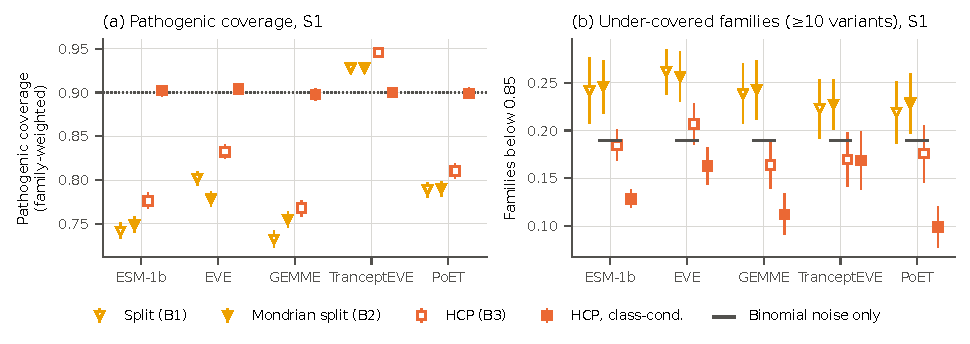
\includegraphics[width=\textwidth]{../figures/fig1_s1_family_coverage.pdf}
\caption{Exchangeable families (S1, $\alpha=0.1$). (a) Family-weighted pathogenic coverage $\Cov_1$ with 95\% family-bootstrap intervals; the dotted line is the target. (b) Fraction of families with at least ten variants whose coverage is below 0.85 (mean and s.d.\ over seeds); the gray dash is the expected fraction if every family had coverage exactly 0.90.}
\label{fig:s1}
\end{figure}

\begin{figure}[h]
\centering
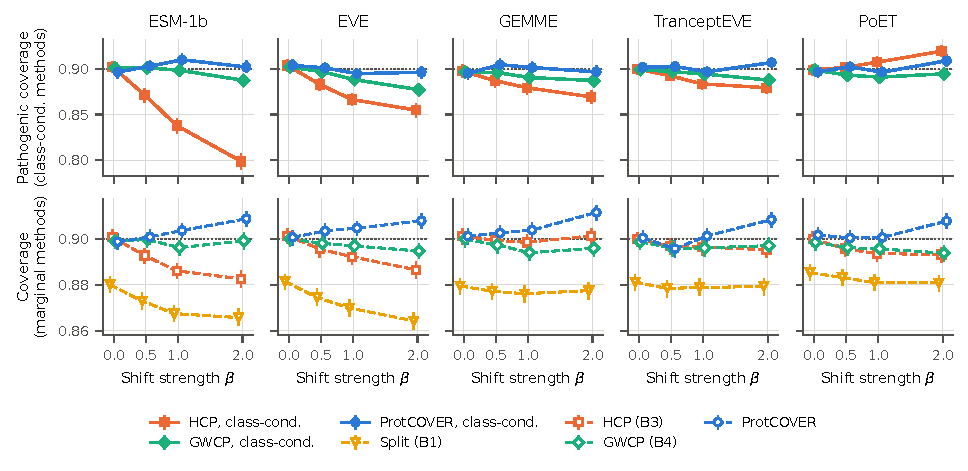
\includegraphics[width=\textwidth]{../figures/fig2_shift_sweep.pdf}
\caption{Class-conditional coverage of both classes under increasing descriptor shift (S2; $\beta=0$ is S1), $\alpha=0.1$, with 95\% family-bootstrap intervals; methods are offset slightly in $\beta$. Mondrian split conformal, far below target, is omitted (Fig.~\ref{fig:s1}).}
\label{fig:shift}
\end{figure}

\begin{figure}[h]
\centering
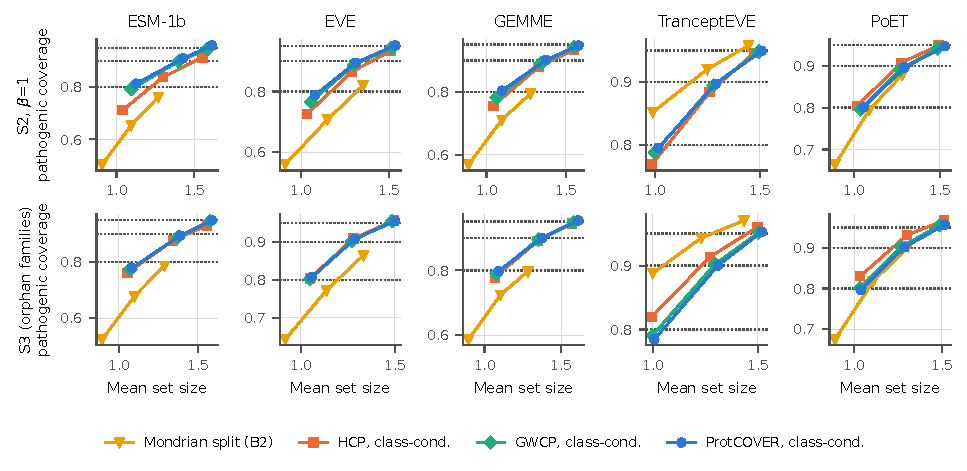
\includegraphics[width=\textwidth]{../figures/fig3_coverage_size.pdf}
\caption{Pathogenic coverage against mean set size for $\alpha\in\{0.2,0.1,0.05\}$ (left to right along each curve), class-conditional methods, on the two shifts defined independently of the descriptors. Dotted lines mark the three targets. A short vertical bar on the 0.90 line marks where a method's curve crosses pathogenic coverage 0.90, found by linear interpolation between its two neighboring levels: the set size the method needs for that coverage, the quantity compared in the last row of Table~\ref{tab:summary}. The methods lie on one coverage-size curve, so a method that covers more also returns larger sets.}
\label{fig:tradeoff}
\end{figure}

\begin{table}[h]
\caption{Family-weighted pathogenic / benign coverage ($\Cov_1$ / $\Cov_0$) of class-conditional methods at $\alpha=0.1$ (target 0.90), per predictor, mean over ten seeds.}
\label{tab:main}
\centering\scriptsize\setlength{\tabcolsep}{3pt}
\begin{tabular}{llccccc}
\toprule
Setting & Method & ESM-1b & EVE & GEMME & TranceptEVE & PoET \\
\midrule
S1 (exchangeable) & Mondrian split (B2) & 0.749 / 0.899 & 0.778 / 0.898 & 0.755 / 0.895 & 0.928 / 0.837 & 0.790 / 0.877 \\
 & HCP (B3) & 0.903 / 0.903 & 0.904 / 0.901 & 0.898 / 0.898 & 0.900 / 0.901 & 0.899 / 0.903 \\
 & GWCP (B4) & 0.902 / 0.901 & 0.902 / 0.899 & 0.897 / 0.897 & 0.900 / 0.900 & 0.899 / 0.901 \\
 & ProtCOVER & \textbf{0.897 / 0.904} & \textbf{0.904 / 0.902} & \textbf{0.895 / 0.899} & \textbf{0.902 / 0.902} & \textbf{0.897 / 0.906} \\
\midrule
S2, $\beta=1$ & Mondrian split (B2) & 0.655 / 0.929 & 0.709 / 0.915 & 0.712 / 0.906 & 0.920 / 0.839 & 0.795 / 0.856 \\
 & HCP (B3) & 0.838 / 0.927 & 0.867 / 0.916 & 0.879 / 0.909 & 0.884 / 0.894 & 0.908 / 0.875 \\
 & GWCP (B4) & 0.899 / 0.904 & 0.888 / 0.909 & 0.891 / 0.904 & 0.895 / 0.894 & 0.891 / 0.897 \\
 & ProtCOVER & \textbf{0.910 / 0.905} & \textbf{0.895 / 0.909} & \textbf{0.902 / 0.908} & \textbf{0.897 / 0.898} & \textbf{0.897 / 0.905} \\
\midrule
S2, $\beta=2$ & Mondrian split (B2) & 0.619 / 0.941 & 0.686 / 0.917 & 0.700 / 0.910 & 0.921 / 0.839 & 0.806 / 0.840 \\
 & HCP (B3) & 0.798 / 0.939 & 0.855 / 0.917 & 0.869 / 0.914 & 0.880 / 0.891 & 0.920 / 0.853 \\
 & GWCP (B4) & 0.888 / 0.905 & 0.877 / 0.906 & 0.887 / 0.897 & 0.888 / 0.889 & 0.895 / 0.873 \\
 & ProtCOVER & \textbf{0.902 / 0.915} & \textbf{0.896 / 0.916} & \textbf{0.898 / 0.915} & \textbf{0.908 / 0.900} & \textbf{0.910 / 0.892} \\
\midrule
S3 (orphan families) & Mondrian split (B2) & 0.678 / 0.915 & 0.772 / 0.895 & 0.724 / 0.903 & 0.943 / 0.823 & 0.817 / 0.854 \\
 & HCP (B3) & 0.876 / 0.908 & 0.909 / 0.899 & 0.890 / 0.905 & 0.914 / 0.892 & 0.931 / 0.879 \\
 & GWCP (B4) & 0.889 / 0.905 & 0.903 / 0.898 & 0.895 / 0.900 & 0.903 / 0.913 & 0.901 / 0.900 \\
 & ProtCOVER & \textbf{0.894 / 0.908} & \textbf{0.907 / 0.901} & \textbf{0.900 / 0.908} & \textbf{0.900 / 0.921} & \textbf{0.901 / 0.910} \\
\bottomrule
\end{tabular}

\end{table}

\begin{table}[h]
\caption{Ablations: pathogenic coverage $\Cov_1$ at $\alpha=0.1$, mean (minimum) over the five predictors, class-conditional versions.}
\label{tab:ablation}
\centering\scriptsize\setlength{\tabcolsep}{3pt}
\begin{tabular}{lcccc}
\toprule
Configuration & S2, $\beta=1$ & S2, $\beta=2$ & S3 & S4 \\
\midrule
\multicolumn{5}{l}{\emph{Components}} \\
(i) family-level calibration (HCP) & 0.875 (0.838) & 0.864 (0.798) & 0.904 (0.876) & 0.904 (0.891) \\
(i)+(ii), conditional on $\hat w$ (ProtCOVER) & 0.901 (0.897) & 0.925 (0.920) & 0.902 (0.890) & 0.914 (0.912) \\
(i)+(ii), conditional on descriptors (ProtCOVER-D) & 0.901 (0.898) & 0.902 (0.890) & 0.905 (0.894) & 0.902 (0.885) \\
(i)+(ii), reweighting by $\hat w$ (ProtCOVER-W) & 0.900 (0.895) & 0.902 (0.896) & 0.900 (0.894) & 0.895 (0.886) \\
(i)+(iii) gate & 0.875 (0.838) & 0.864 (0.798) & 0.904 (0.876) & 0.904 (0.891) \\
ProtCOVER-W + (iii) gate & 0.900 (0.895) & 0.904 (0.898) & 0.901 (0.894) & 0.895 (0.886) \\
(ii) without (i): variant-level weighting & 0.789 (0.740) & 0.787 (0.723) & 0.807 (0.740) & 0.798 (0.737) \\
\multicolumn{5}{l}{\emph{Descriptors for $\hat w$ (ProtCOVER-W)}} \\
sequence similarity only & 0.871 (0.850) & 0.853 (0.799) & 0.899 (0.892) & 0.906 (0.903) \\
alignment depth only & 0.899 (0.892) & 0.901 (0.872) & 0.899 (0.878) & 0.903 (0.893) \\
embedding distance only & 0.879 (0.845) & 0.866 (0.806) & 0.904 (0.872) & 0.895 (0.882) \\
the three support groups & 0.900 (0.894) & 0.904 (0.898) & 0.900 (0.894) & 0.896 (0.887) \\
main set + predictor score summaries & 0.903 (0.894) & 0.898 (0.889) & 0.902 (0.895) & 0.894 (0.887) \\
\multicolumn{5}{l}{\emph{Weight clipping $c$ (default 20; ProtCOVER-W)}} \\
$c=5$ & 0.899 (0.894) & 0.889 (0.870) & 0.900 (0.892) & 0.904 (0.897) \\
$c=100$ & 0.900 (0.895) & 0.908 (0.904) & 0.901 (0.894) & 0.883 (0.874) \\
no clipping & 0.900 (0.895) & 0.908 (0.904) & 0.901 (0.894) & 0.837 (0.779) \\
\bottomrule
\end{tabular}

\end{table}

\begin{table}[h]
\caption{Pooling, feature classes and the share of calibration families that fit $\hat w$, over the \revNCells{} shifted cells at $\alpha=0.1$ (class-conditional versions). Shortfall: worse-class shortfall, mean (maximum) over cells. Set size: mean. s.d.\ $\Cov_1$: seed-to-seed standard deviation of pathogenic coverage, mean over cells. Abstention: largest fraction of test families with an infinite threshold in any cell. Margin: cells where ProtCOVER's shortfall is smaller / larger than the variant's by more than 0.01. Paired: cells where ProtCOVER's worse-class coverage is higher / lower than the variant's with a paired 95\% interval that excludes zero. Variants were declared in the configuration before they were run.}
\label{tab:review}
\centering\scriptsize\setlength{\tabcolsep}{3pt}
\begin{tabular}{lcccccc}
\toprule
Variant & Shortfall & Set size & s.d.\ $\Cov_1$ & Abstention & Margin & Paired \\
\midrule
ProtCOVER, features $(1,\hat w)$, ratio fitted on a third (default) & 0.001 (0.010) & 1.357 & 0.018 & 0.3\% & - & - \\
\quad one variant per family and class (Gibbs et al.) & 0.002 (0.016) & 1.355 & 0.020 & 0.3\% & 1/0 & 7/1 \\
\quad features $(1,\hat w,d)$ & 0.000 (0.003) & 1.380 & 0.017 & 0.3\% & 0/0 & 0/18 \\
\quad ratio fitted on 20\% of calibration families & 0.002 (0.015) & 1.349 & 0.019 & 1.1\% & 0/0 & 13/1 \\
\quad ratio fitted on 50\% & 0.001 (0.008) & 1.375 & 0.019 & 1.5\% & 0/0 & 3/10 \\
ProtCOVER-D, features $(1,d)$ (default) & 0.003 (0.015) & 1.324 & 0.017 & 0.0\% & 3/0 & - \\
\quad features $(1,d,d^2)$ & 0.001 (0.007) & 1.338 & 0.016 & 0.4\% & 0/0 & 6/8 \\
ProtCOVER-W, ratio fitted on a third (default) & 0.003 (0.014) & 1.335 & 0.023 & 0.0\% & 2/0 & - \\
\quad ratio fitted on 20\% & 0.005 (0.019) & 1.331 & 0.024 & 0.0\% & 3/0 & - \\
\quad ratio fitted on 50\% & 0.003 (0.020) & 1.349 & 0.025 & 0.0\% & 3/0 & - \\
\bottomrule
\end{tabular}

\end{table}

\begin{figure}[h]
\centering
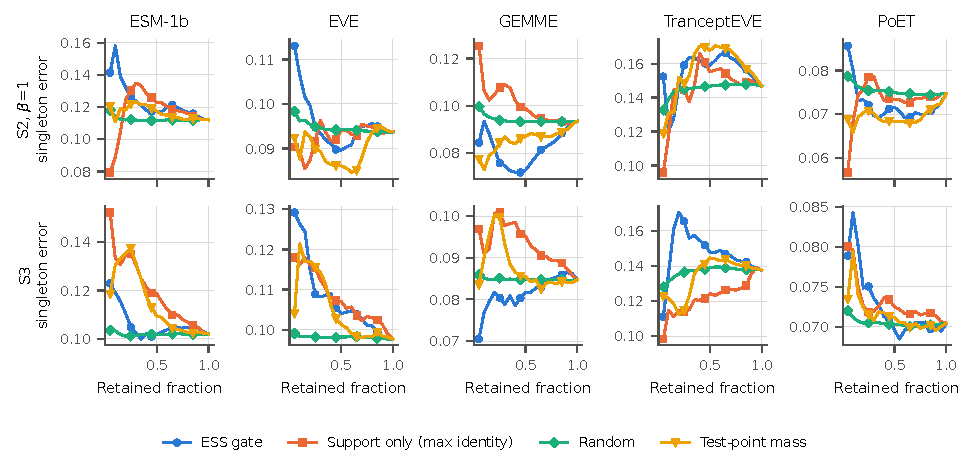
\includegraphics[width=\textwidth]{../figures/fig4_risk_coverage.pdf}
\caption{Risk-coverage of abstention rules applied to ProtCOVER-W's class-conditional sets ($\alpha=0.1$, mean over seeds): error of retained singleton sets as whole families are abstained in order of the score. Random abstention is averaged over 100 random family orders. The gate's decision depends only on label-free quantities, so it abstains on the same families whichever variant of (ii) it wraps.}
\label{fig:risk}
\end{figure}

Tables~\ref{tab:pairedpath}--\ref{tab:effsingerr} give paired differences between ProtCOVER and HCP, GWCP and ProtCOVER-W (class-conditional versions, $\alpha=0.1$, mean over seeds) with 95\% paired family-bootstrap intervals, which are conditional on the splits. Singleton error is the fraction of single-label sets that exclude the true label.

\begin{table}[h]
\caption{Paired differences in pathogenic coverage $\Cov_1$: ProtCOVER minus each baseline.}
\label{tab:pairedpath}
\centering\footnotesize\setlength{\tabcolsep}{3.5pt}
\begin{tabular}{llccc}
\toprule
 & & \multicolumn{3}{c}{$\Cov_1$ (pathogenic)} \\
\cmidrule(lr){3-5}
Setting & Predictor & $-$ HCP & $-$ GWCP & $-$ ProtCOVER-W \\
\midrule
S1 & ESM-1b & +0.001 [$-$0.003, +0.005] & +0.002 [$-$0.002, +0.006] & +0.006 [+0.003, +0.011] \\
 & EVE & $-$0.001 [$-$0.004, +0.001] & +0.001 [$-$0.002, +0.003] & $-$0.001 [$-$0.004, +0.001] \\
 & GEMME & +0.003 [$-$0.001, +0.006] & +0.004 [+0.001, +0.007] & +0.005 [+0.002, +0.009] \\
 & TranceptEVE & +0.005 [+0.003, +0.008] & +0.006 [+0.003, +0.009] & +0.004 [+0.001, +0.007] \\
 & PoET & +0.002 [$-$0.001, +0.005] & +0.002 [$-$0.001, +0.005] & +0.004 [+0.001, +0.007] \\
\midrule
S2, $\beta=1$ & ESM-1b & +0.071 [+0.065, +0.078] & +0.010 [+0.004, +0.017] & $-$0.001 [$-$0.008, +0.005] \\
 & EVE & +0.031 [+0.027, +0.036] & +0.009 [+0.005, +0.013] & +0.002 [$-$0.002, +0.007] \\
 & GEMME & +0.023 [+0.020, +0.027] & +0.012 [+0.008, +0.016] & +0.001 [$-$0.002, +0.005] \\
 & TranceptEVE & +0.015 [+0.012, +0.019] & +0.005 [+0.002, +0.008] & +0.002 [$-$0.000, +0.005] \\
 & PoET & $-$0.008 [$-$0.011, $-$0.006] & +0.008 [+0.005, +0.010] & +0.003 [+0.000, +0.005] \\
\midrule
S2, $\beta=2$ & ESM-1b & +0.131 [+0.124, +0.139] & +0.042 [+0.035, +0.049] & +0.027 [+0.021, +0.034] \\
 & EVE & +0.069 [+0.064, +0.075] & +0.047 [+0.042, +0.053] & +0.028 [+0.024, +0.032] \\
 & GEMME & +0.052 [+0.047, +0.057] & +0.034 [+0.029, +0.039] & +0.025 [+0.020, +0.029] \\
 & TranceptEVE & +0.052 [+0.048, +0.056] & +0.043 [+0.039, +0.048] & +0.024 [+0.021, +0.028] \\
 & PoET & $-$0.000 [$-$0.003, +0.003] & +0.025 [+0.021, +0.029] & +0.010 [+0.007, +0.013] \\
\midrule
S3 & ESM-1b & +0.014 [+0.011, +0.017] & +0.001 [$-$0.002, +0.004] & $-$0.004 [$-$0.006, $-$0.001] \\
 & EVE & $-$0.002 [$-$0.004, +0.000] & +0.004 [+0.002, +0.006] & +0.000 [$-$0.001, +0.002] \\
 & GEMME & +0.010 [+0.007, +0.012] & +0.005 [+0.002, +0.007] & +0.000 [$-$0.002, +0.002] \\
 & TranceptEVE & $-$0.012 [$-$0.014, $-$0.009] & $-$0.001 [$-$0.003, +0.002] & +0.002 [+0.000, +0.004] \\
 & PoET & $-$0.021 [$-$0.024, $-$0.018] & +0.009 [+0.007, +0.012] & +0.009 [+0.007, +0.012] \\
\midrule
S4 & ESM-1b & +0.021 [+0.018, +0.025] & +0.016 [+0.013, +0.020] & +0.026 [+0.022, +0.031] \\
 & EVE & +0.008 [+0.006, +0.011] & +0.015 [+0.012, +0.019] & +0.018 [+0.015, +0.022] \\
 & GEMME & +0.012 [+0.009, +0.014] & +0.015 [+0.012, +0.018] & +0.012 [+0.009, +0.014] \\
 & TranceptEVE & +0.004 [+0.002, +0.006] & +0.012 [+0.009, +0.014] & +0.023 [+0.020, +0.026] \\
 & PoET & +0.004 [+0.002, +0.007] & +0.016 [+0.013, +0.018] & +0.016 [+0.013, +0.019] \\
\bottomrule
\end{tabular}

\end{table}

\begin{table}[h]
\caption{Paired differences in benign coverage $\Cov_0$: ProtCOVER minus each baseline.}
\label{tab:pairedbenign}
\centering\footnotesize\setlength{\tabcolsep}{3.5pt}
\begin{tabular}{llccc}
\toprule
 & & \multicolumn{3}{c}{$\Cov_0$ (benign)} \\
\cmidrule(lr){3-5}
Setting & Predictor & $-$ HCP & $-$ GWCP & $-$ ProtCOVER-W \\
\midrule
S1 & ESM-1b & +0.002 [$-$0.000, +0.004] & +0.004 [+0.002, +0.006] & +0.001 [$-$0.001, +0.003] \\
 & EVE & +0.003 [+0.002, +0.005] & +0.005 [+0.004, +0.007] & +0.003 [+0.001, +0.004] \\
 & GEMME & +0.001 [$-$0.000, +0.003] & +0.003 [+0.001, +0.004] & +0.001 [$-$0.000, +0.002] \\
 & TranceptEVE & +0.004 [+0.002, +0.007] & +0.005 [+0.003, +0.008] & +0.003 [+0.001, +0.006] \\
 & PoET & +0.004 [+0.001, +0.007] & +0.006 [+0.004, +0.009] & +0.001 [$-$0.002, +0.004] \\
\midrule
S2, $\beta=1$ & ESM-1b & $-$0.016 [$-$0.019, $-$0.015] & +0.006 [+0.004, +0.009] & +0.006 [+0.004, +0.008] \\
 & EVE & $-$0.001 [$-$0.003, $-$0.000] & +0.006 [+0.005, +0.008] & +0.005 [+0.004, +0.007] \\
 & GEMME & +0.002 [+0.001, +0.004] & +0.008 [+0.006, +0.010] & +0.004 [+0.002, +0.005] \\
 & TranceptEVE & +0.012 [+0.010, +0.014] & +0.011 [+0.010, +0.013] & +0.007 [+0.006, +0.009] \\
 & PoET & +0.033 [+0.029, +0.036] & +0.010 [+0.007, +0.013] & +0.002 [$-$0.001, +0.006] \\
\midrule
S2, $\beta=2$ & ESM-1b & $-$0.020 [$-$0.022, $-$0.018] & +0.014 [+0.012, +0.016] & +0.004 [+0.001, +0.006] \\
 & EVE & +0.011 [+0.009, +0.013] & +0.021 [+0.019, +0.023] & +0.012 [+0.010, +0.014] \\
 & GEMME & +0.011 [+0.009, +0.013] & +0.028 [+0.026, +0.031] & +0.010 [+0.008, +0.012] \\
 & TranceptEVE & +0.030 [+0.027, +0.034] & +0.032 [+0.029, +0.036] & +0.022 [+0.019, +0.025] \\
 & PoET & +0.073 [+0.069, +0.078] & +0.053 [+0.049, +0.058] & +0.035 [+0.031, +0.039] \\
\midrule
S3 & ESM-1b & +0.002 [+0.000, +0.003] & +0.005 [+0.004, +0.006] & +0.002 [+0.001, +0.003] \\
 & EVE & +0.004 [+0.003, +0.005] & +0.004 [+0.003, +0.005] & +0.001 [+0.000, +0.002] \\
 & GEMME & +0.004 [+0.003, +0.005] & +0.009 [+0.007, +0.010] & +0.001 [+0.000, +0.002] \\
 & TranceptEVE & +0.025 [+0.023, +0.028] & +0.004 [+0.002, +0.007] & $-$0.004 [$-$0.005, $-$0.002] \\
 & PoET & +0.026 [+0.023, +0.029] & +0.004 [+0.002, +0.006] & $-$0.005 [$-$0.007, $-$0.003] \\
\midrule
S4 & ESM-1b & +0.006 [+0.004, +0.008] & +0.003 [+0.001, +0.006] & $-$0.000 [$-$0.002, +0.002] \\
 & EVE & +0.003 [+0.001, +0.004] & +0.001 [$-$0.001, +0.002] & $-$0.010 [$-$0.012, $-$0.008] \\
 & GEMME & +0.008 [+0.006, +0.009] & +0.010 [+0.008, +0.012] & +0.014 [+0.012, +0.017] \\
 & TranceptEVE & +0.016 [+0.014, +0.019] & +0.009 [+0.006, +0.011] & $-$0.010 [$-$0.012, $-$0.007] \\
 & PoET & +0.020 [+0.018, +0.023] & +0.014 [+0.011, +0.017] & $-$0.003 [$-$0.005, +0.000] \\
\bottomrule
\end{tabular}

\end{table}

\begin{table}[h]
\caption{Paired differences in mean set size (variant-weighted): ProtCOVER minus each baseline.}
\label{tab:effsize}
\centering\footnotesize\setlength{\tabcolsep}{3.5pt}
\begin{tabular}{llccc}
\toprule
 & & \multicolumn{3}{c}{Mean set size} \\
\cmidrule(lr){3-5}
Setting & Predictor & $-$ HCP & $-$ GWCP & $-$ ProtCOVER-W \\
\midrule
S1 & ESM-1b & $-$0.013 [$-$0.019, $-$0.006] & $-$0.009 [$-$0.015, $-$0.002] & $-$0.003 [$-$0.008, +0.004] \\
 & EVE & +0.010 [+0.006, +0.015] & +0.016 [+0.012, +0.021] & +0.006 [+0.003, +0.010] \\
 & GEMME & $-$0.004 [$-$0.008, $-$0.000] & $-$0.001 [$-$0.005, +0.003] & $-$0.001 [$-$0.005, +0.003] \\
 & TranceptEVE & +0.010 [$-$0.000, +0.019] & +0.013 [+0.003, +0.022] & +0.003 [$-$0.007, +0.012] \\
 & PoET & +0.009 [+0.002, +0.015] & +0.013 [+0.006, +0.019] & +0.009 [+0.002, +0.016] \\
\midrule
S2, $\beta=1$ & ESM-1b & +0.079 [+0.069, +0.091] & $-$0.020 [$-$0.031, $-$0.010] & $-$0.051 [$-$0.061, $-$0.040] \\
 & EVE & +0.041 [+0.035, +0.047] & +0.031 [+0.025, +0.037] & +0.021 [+0.016, +0.027] \\
 & GEMME & +0.047 [+0.041, +0.053] & +0.030 [+0.025, +0.037] & $-$0.003 [$-$0.008, +0.002] \\
 & TranceptEVE & +0.052 [+0.046, +0.059] & +0.034 [+0.027, +0.042] & +0.022 [+0.016, +0.029] \\
 & PoET & +0.020 [+0.014, +0.026] & +0.026 [+0.020, +0.033] & +0.000 [$-$0.005, +0.007] \\
\midrule
S2, $\beta=2$ & ESM-1b & +0.188 [+0.173, +0.204] & +0.055 [+0.042, +0.069] & +0.012 [+0.001, +0.024] \\
 & EVE & +0.170 [+0.158, +0.184] & +0.159 [+0.148, +0.173] & +0.114 [+0.105, +0.126] \\
 & GEMME & +0.150 [+0.138, +0.163] & +0.123 [+0.112, +0.135] & +0.080 [+0.073, +0.090] \\
 & TranceptEVE & +0.220 [+0.206, +0.237] & +0.206 [+0.192, +0.223] & +0.154 [+0.142, +0.168] \\
 & PoET & +0.149 [+0.137, +0.163] & +0.174 [+0.161, +0.189] & +0.117 [+0.106, +0.129] \\
\midrule
S3 & ESM-1b & +0.031 [+0.027, +0.037] & $-$0.001 [$-$0.005, +0.005] & $-$0.015 [$-$0.020, $-$0.010] \\
 & EVE & +0.012 [+0.010, +0.013] & +0.018 [+0.016, +0.020] & +0.006 [+0.005, +0.007] \\
 & GEMME & +0.029 [+0.026, +0.032] & +0.024 [+0.020, +0.027] & $-$0.001 [$-$0.004, +0.002] \\
 & TranceptEVE & +0.031 [+0.027, +0.035] & +0.007 [+0.003, +0.011] & $-$0.006 [$-$0.009, $-$0.003] \\
 & PoET & $-$0.005 [$-$0.009, $-$0.002] & +0.027 [+0.025, +0.030] & +0.010 [+0.007, +0.013] \\
\midrule
S4 & ESM-1b & +0.040 [+0.033, +0.047] & +0.035 [+0.027, +0.042] & +0.047 [+0.039, +0.055] \\
 & EVE & +0.037 [+0.029, +0.047] & +0.042 [+0.034, +0.051] & +0.005 [$-$0.001, +0.012] \\
 & GEMME & +0.052 [+0.043, +0.064] & +0.063 [+0.053, +0.074] & +0.048 [+0.039, +0.058] \\
 & TranceptEVE & +0.043 [+0.036, +0.050] & +0.044 [+0.036, +0.052] & +0.022 [+0.013, +0.031] \\
 & PoET & +0.041 [+0.034, +0.048] & +0.058 [+0.052, +0.065] & +0.028 [+0.023, +0.035] \\
\bottomrule
\end{tabular}

\end{table}

\begin{table}[h]
\caption{Paired differences in singleton error: ProtCOVER minus each baseline.}
\label{tab:effsingerr}
\centering\footnotesize\setlength{\tabcolsep}{3.5pt}
\begin{tabular}{llccc}
\toprule
 & & \multicolumn{3}{c}{Singleton error} \\
\cmidrule(lr){3-5}
Setting & Predictor & $-$ HCP & $-$ GWCP & $-$ ProtCOVER-W \\
\midrule
S1 & ESM-1b & $-$0.002 [$-$0.005, +0.001] & $-$0.003 [$-$0.006, $-$0.001] & $-$0.001 [$-$0.003, +0.002] \\
 & EVE & +0.002 [+0.001, +0.005] & +0.001 [$-$0.001, +0.003] & +0.003 [+0.001, +0.005] \\
 & GEMME & +0.000 [$-$0.002, +0.002] & $-$0.001 [$-$0.003, +0.001] & +0.001 [$-$0.001, +0.002] \\
 & TranceptEVE & +0.001 [$-$0.009, +0.012] & +0.000 [$-$0.009, +0.011] & +0.002 [$-$0.008, +0.013] \\
 & PoET & +0.008 [+0.005, +0.011] & +0.007 [+0.004, +0.010] & +0.008 [+0.006, +0.011] \\
\midrule
S2, $\beta=1$ & ESM-1b & +0.007 [+0.004, +0.010] & $-$0.010 [$-$0.014, $-$0.007] & $-$0.011 [$-$0.015, $-$0.007] \\
 & EVE & $-$0.000 [$-$0.002, +0.001] & $-$0.001 [$-$0.002, +0.001] & +0.001 [$-$0.001, +0.002] \\
 & GEMME & +0.002 [+0.001, +0.004] & $-$0.002 [$-$0.003, $-$0.001] & $-$0.000 [$-$0.002, +0.001] \\
 & TranceptEVE & +0.001 [$-$0.002, +0.004] & +0.008 [+0.004, +0.012] & +0.010 [+0.006, +0.014] \\
 & PoET & $-$0.013 [$-$0.015, $-$0.011] & $-$0.004 [$-$0.006, $-$0.002] & +0.000 [$-$0.002, +0.002] \\
\midrule
S2, $\beta=2$ & ESM-1b & +0.010 [+0.006, +0.015] & $-$0.014 [$-$0.018, $-$0.010] & $-$0.005 [$-$0.008, $-$0.001] \\
 & EVE & $-$0.004 [$-$0.006, $-$0.001] & $-$0.007 [$-$0.009, $-$0.004] & +0.001 [$-$0.001, +0.004] \\
 & GEMME & +0.002 [$-$0.001, +0.005] & $-$0.014 [$-$0.017, $-$0.010] & +0.000 [$-$0.003, +0.003] \\
 & TranceptEVE & +0.004 [$-$0.003, +0.010] & +0.008 [+0.000, +0.015] & +0.018 [+0.011, +0.024] \\
 & PoET & $-$0.026 [$-$0.029, $-$0.022] & $-$0.018 [$-$0.021, $-$0.015] & $-$0.007 [$-$0.010, $-$0.005] \\
\midrule
S3 & ESM-1b & $-$0.002 [$-$0.003, $-$0.001] & $-$0.005 [$-$0.007, $-$0.004] & $-$0.004 [$-$0.005, $-$0.002] \\
 & EVE & $-$0.003 [$-$0.004, $-$0.002] & $-$0.004 [$-$0.005, $-$0.003] & $-$0.001 [$-$0.002, $-$0.000] \\
 & GEMME & $-$0.002 [$-$0.004, $-$0.001] & $-$0.004 [$-$0.006, $-$0.003] & $-$0.001 [$-$0.003, +0.000] \\
 & TranceptEVE & +0.004 [+0.001, +0.008] & $-$0.001 [$-$0.003, +0.002] & $-$0.001 [$-$0.003, +0.000] \\
 & PoET & $-$0.004 [$-$0.006, $-$0.003] & $-$0.001 [$-$0.002, +0.001] & +0.003 [+0.001, +0.004] \\
\midrule
S4 & ESM-1b & $-$0.002 [$-$0.004, +0.000] & $-$0.001 [$-$0.003, +0.001] & $-$0.001 [$-$0.003, +0.002] \\
 & EVE & +0.001 [$-$0.001, +0.002] & $-$0.001 [$-$0.002, +0.000] & +0.001 [$-$0.000, +0.003] \\
 & GEMME & +0.002 [+0.001, +0.003] & $-$0.000 [$-$0.002, +0.001] & $-$0.002 [$-$0.004, $-$0.000] \\
 & TranceptEVE & $-$0.004 [$-$0.011, +0.001] & $-$0.013 [$-$0.021, $-$0.006] & $-$0.024 [$-$0.032, $-$0.016] \\
 & PoET & $-$0.005 [$-$0.006, $-$0.003] & $-$0.004 [$-$0.006, $-$0.003] & +0.001 [$-$0.001, +0.003] \\
\bottomrule
\end{tabular}

\end{table}

Tables~\ref{tab:full10}--\ref{tab:full20} report every method, marginal (cc $=$ no) and class-conditional (cc $=$ yes), averaged over the five predictors: family-weighted coverage $\Cov$, variant-weighted coverage, $\Cov_1$, $\Cov_0$, mean set size, singleton rate, the fraction of families with at least ten variants whose coverage is below $1-\alpha-0.05$, and the fraction of test families on which the method abstained. Per-predictor values with bootstrap intervals, and the summaries of every sensitivity, stress and external run, are in \path{results/} of the code repository.

{\footnotesize\setlength{\tabcolsep}{2.5pt}
\begin{tabular}{llccccccccc}
\toprule
Setting & Method & cc & $\Cov$ & var.-w. & $\Cov_1$ & $\Cov_0$ & size & single. & under-cov. & abst. \\
\midrule
S1 (exchangeable) & Split (B1/B2) & no & 0.882 & 0.899 & 0.798 & 0.884 & 1.143 & 0.857 & 0.237 & 0.000 \\
 & Split (B1/B2) & yes & 0.881 & 0.898 & 0.800 & 0.881 & 1.142 & 0.858 & 0.240 & 0.000 \\
 & HCP (B3) & no & 0.901 & 0.918 & 0.827 & 0.903 & 1.204 & 0.796 & 0.180 & 0.000 \\
 & HCP (B3) & yes & 0.922 & 0.929 & 0.901 & 0.901 & 1.304 & 0.696 & 0.134 & 0.000 \\
 & Subsample once (B3) & no & 0.900 & 0.918 & 0.828 & 0.902 & 1.204 & 0.796 & 0.180 & 0.000 \\
 & Subsample once (B3) & yes & 0.922 & 0.929 & 0.901 & 0.900 & 1.305 & 0.695 & 0.136 & 0.000 \\
 & Repeated subsample (B3) & no & 0.901 & 0.918 & 0.826 & 0.903 & 1.205 & 0.795 & 0.180 & 0.000 \\
 & Repeated subsample (B3) & yes & 0.923 & 0.929 & 0.901 & 0.901 & 1.305 & 0.695 & 0.134 & 0.000 \\
 & GWCP (B4) & no & 0.899 & 0.917 & 0.824 & 0.901 & 1.199 & 0.801 & 0.185 & 0.000 \\
 & GWCP (B4) & yes & 0.921 & 0.928 & 0.900 & 0.899 & 1.300 & 0.700 & 0.136 & 0.000 \\
 & ProtCOVER (i)+(ii) & no & 0.900 & 0.918 & 0.826 & 0.903 & 1.204 & 0.796 & 0.181 & 0.000 \\
 & ProtCOVER (i)+(ii) & yes & 0.923 & 0.930 & 0.899 & 0.902 & 1.303 & 0.697 & 0.133 & 0.000 \\
 & ProtCOVER (i)+(iii) & no & 0.901 & 0.918 & 0.827 & 0.903 & 1.204 & 0.796 & 0.180 & 0.000 \\
 & ProtCOVER (i)+(iii) & yes & 0.923 & 0.929 & 0.901 & 0.901 & 1.304 & 0.696 & 0.134 & 0.000 \\
 & ProtCOVER full & no & 0.901 & 0.918 & 0.826 & 0.903 & 1.204 & 0.796 & 0.180 & 0.000 \\
 & ProtCOVER full & yes & 0.923 & 0.930 & 0.899 & 0.903 & 1.304 & 0.696 & 0.133 & 0.000 \\
 & Support-only abst. (B5) & no & 0.901 & 0.918 & 0.826 & 0.903 & 1.204 & 0.796 & 0.181 & 0.000 \\
 & Support-only abst. (B5) & yes & 0.923 & 0.930 & 0.899 & 0.902 & 1.304 & 0.696 & 0.133 & 0.000 \\
 & Random abst. (B5) & no & 0.901 & 0.918 & 0.826 & 0.903 & 1.204 & 0.796 & 0.180 & 0.000 \\
 & Random abst. (B5) & yes & 0.923 & 0.930 & 0.899 & 0.902 & 1.304 & 0.696 & 0.133 & 0.000 \\
\midrule
S2, $\beta=1$ & Split (B1/B2) & no & 0.875 & 0.893 & 0.772 & 0.883 & 1.137 & 0.863 & 0.252 & 0.000 \\
 & Split (B1/B2) & yes & 0.873 & 0.891 & 0.758 & 0.889 & 1.137 & 0.863 & 0.255 & 0.000 \\
 & HCP (B3) & no & 0.893 & 0.912 & 0.800 & 0.901 & 1.195 & 0.805 & 0.200 & 0.000 \\
 & HCP (B3) & yes & 0.917 & 0.925 & 0.875 & 0.904 & 1.291 & 0.709 & 0.147 & 0.000 \\
 & Subsample once (B3) & no & 0.893 & 0.912 & 0.800 & 0.902 & 1.195 & 0.805 & 0.200 & 0.000 \\
 & Subsample once (B3) & yes & 0.918 & 0.926 & 0.877 & 0.904 & 1.294 & 0.706 & 0.146 & 0.000 \\
 & Repeated subsample (B3) & no & 0.893 & 0.912 & 0.800 & 0.901 & 1.195 & 0.805 & 0.200 & 0.000 \\
 & Repeated subsample (B3) & yes & 0.917 & 0.925 & 0.875 & 0.904 & 1.290 & 0.710 & 0.147 & 0.000 \\
 & GWCP (B4) & no & 0.896 & 0.914 & 0.805 & 0.903 & 1.202 & 0.798 & 0.195 & 0.000 \\
 & GWCP (B4) & yes & 0.921 & 0.928 & 0.893 & 0.902 & 1.318 & 0.682 & 0.140 & 0.000 \\
 & ProtCOVER (i)+(ii) & no & 0.903 & 0.921 & 0.818 & 0.909 & 1.227 & 0.773 & 0.176 & 0.000 \\
 & ProtCOVER (i)+(ii) & yes & 0.925 & 0.931 & 0.900 & 0.905 & 1.340 & 0.660 & 0.130 & 0.000 \\
 & ProtCOVER (i)+(iii) & no & 0.893 & 0.912 & 0.800 & 0.901 & 1.195 & 0.805 & 0.200 & 0.000 \\
 & ProtCOVER (i)+(iii) & yes & 0.917 & 0.925 & 0.875 & 0.904 & 1.291 & 0.709 & 0.147 & 0.000 \\
 & ProtCOVER full & no & 0.903 & 0.921 & 0.818 & 0.909 & 1.227 & 0.773 & 0.176 & 0.000 \\
 & ProtCOVER full & yes & 0.925 & 0.931 & 0.900 & 0.905 & 1.340 & 0.660 & 0.129 & 0.000 \\
 & Support-only abst. (B5) & no & 0.903 & 0.921 & 0.818 & 0.909 & 1.227 & 0.773 & 0.176 & 0.000 \\
 & Support-only abst. (B5) & yes & 0.925 & 0.931 & 0.900 & 0.905 & 1.341 & 0.659 & 0.130 & 0.000 \\
 & Random abst. (B5) & no & 0.903 & 0.921 & 0.818 & 0.909 & 1.227 & 0.773 & 0.176 & 0.000 \\
 & Random abst. (B5) & yes & 0.925 & 0.931 & 0.900 & 0.905 & 1.341 & 0.659 & 0.130 & 0.000 \\
\midrule
S2, $\beta=2$ & Split (B1/B2) & no & 0.874 & 0.892 & 0.764 & 0.883 & 1.136 & 0.864 & 0.255 & 0.000 \\
 & Split (B1/B2) & yes & 0.871 & 0.890 & 0.746 & 0.889 & 1.136 & 0.864 & 0.259 & 0.000 \\
 & HCP (B3) & no & 0.892 & 0.911 & 0.793 & 0.900 & 1.192 & 0.808 & 0.204 & 0.000 \\
 & HCP (B3) & yes & 0.914 & 0.923 & 0.864 & 0.903 & 1.283 & 0.717 & 0.156 & 0.000 \\
 & Subsample once (B3) & no & 0.889 & 0.909 & 0.792 & 0.896 & 1.187 & 0.813 & 0.211 & 0.000 \\
 & Subsample once (B3) & yes & 0.912 & 0.922 & 0.863 & 0.901 & 1.279 & 0.721 & 0.159 & 0.000 \\
 & Repeated subsample (B3) & no & 0.891 & 0.911 & 0.792 & 0.900 & 1.192 & 0.808 & 0.204 & 0.000 \\
 & Repeated subsample (B3) & yes & 0.914 & 0.923 & 0.864 & 0.903 & 1.283 & 0.717 & 0.156 & 0.000 \\
 & GWCP (B4) & no & 0.896 & 0.915 & 0.801 & 0.904 & 1.212 & 0.788 & 0.196 & 0.000 \\
 & GWCP (B4) & yes & 0.915 & 0.923 & 0.887 & 0.894 & 1.315 & 0.685 & 0.159 & 0.000 \\
 & ProtCOVER (i)+(ii) & no & 0.909 & 0.927 & 0.826 & 0.914 & 1.260 & 0.740 & 0.161 & 0.000 \\
 & ProtCOVER (i)+(ii) & yes & 0.927 & 0.935 & 0.902 & 0.907 & 1.363 & 0.637 & 0.127 & 0.000 \\
 & ProtCOVER (i)+(iii) & no & 0.892 & 0.911 & 0.793 & 0.900 & 1.192 & 0.808 & 0.204 & 0.000 \\
 & ProtCOVER (i)+(iii) & yes & 0.914 & 0.923 & 0.864 & 0.903 & 1.283 & 0.717 & 0.156 & 0.000 \\
 & ProtCOVER full & no & 0.909 & 0.927 & 0.827 & 0.914 & 1.264 & 0.736 & 0.161 & 0.004 \\
 & ProtCOVER full & yes & 0.928 & 0.936 & 0.904 & 0.908 & 1.372 & 0.628 & 0.125 & 0.022 \\
 & Support-only abst. (B5) & no & 0.909 & 0.927 & 0.827 & 0.914 & 1.263 & 0.737 & 0.160 & 0.004 \\
 & Support-only abst. (B5) & yes & 0.928 & 0.936 & 0.904 & 0.909 & 1.375 & 0.625 & 0.125 & 0.022 \\
 & Random abst. (B5) & no & 0.909 & 0.928 & 0.827 & 0.915 & 1.264 & 0.736 & 0.160 & 0.004 \\
 & Random abst. (B5) & yes & 0.928 & 0.936 & 0.904 & 0.909 & 1.375 & 0.625 & 0.125 & 0.022 \\
\midrule
S3 (orphan families) & Split (B1/B2) & no & 0.875 & 0.891 & 0.789 & 0.878 & 1.137 & 0.863 & 0.254 & 0.000 \\
 & Split (B1/B2) & yes & 0.874 & 0.890 & 0.787 & 0.878 & 1.135 & 0.865 & 0.251 & 0.000 \\
 & HCP (B3) & no & 0.897 & 0.913 & 0.821 & 0.899 & 1.204 & 0.796 & 0.193 & 0.000 \\
 & HCP (B3) & yes & 0.922 & 0.931 & 0.904 & 0.896 & 1.308 & 0.692 & 0.129 & 0.000 \\
 & Subsample once (B3) & no & 0.896 & 0.912 & 0.820 & 0.898 & 1.204 & 0.796 & 0.195 & 0.000 \\
 & Subsample once (B3) & yes & 0.922 & 0.931 & 0.904 & 0.896 & 1.309 & 0.691 & 0.128 & 0.000 \\
 & Repeated subsample (B3) & no & 0.896 & 0.912 & 0.821 & 0.899 & 1.203 & 0.797 & 0.194 & 0.000 \\
 & Repeated subsample (B3) & yes & 0.922 & 0.931 & 0.904 & 0.896 & 1.308 & 0.692 & 0.129 & 0.000 \\
 & GWCP (B4) & no & 0.901 & 0.917 & 0.827 & 0.903 & 1.220 & 0.780 & 0.182 & 0.000 \\
 & GWCP (B4) & yes & 0.924 & 0.931 & 0.898 & 0.903 & 1.312 & 0.688 & 0.128 & 0.000 \\
 & ProtCOVER (i)+(ii) & no & 0.905 & 0.922 & 0.834 & 0.908 & 1.238 & 0.762 & 0.170 & 0.000 \\
 & ProtCOVER (i)+(ii) & yes & 0.928 & 0.934 & 0.900 & 0.910 & 1.329 & 0.671 & 0.120 & 0.000 \\
 & ProtCOVER (i)+(iii) & no & 0.897 & 0.913 & 0.821 & 0.899 & 1.204 & 0.796 & 0.193 & 0.000 \\
 & ProtCOVER (i)+(iii) & yes & 0.922 & 0.931 & 0.904 & 0.897 & 1.309 & 0.691 & 0.129 & 0.003 \\
 & ProtCOVER full & no & 0.905 & 0.922 & 0.834 & 0.908 & 1.238 & 0.762 & 0.170 & 0.000 \\
 & ProtCOVER full & yes & 0.928 & 0.934 & 0.901 & 0.910 & 1.331 & 0.669 & 0.120 & 0.004 \\
 & Support-only abst. (B5) & no & 0.905 & 0.922 & 0.834 & 0.908 & 1.238 & 0.762 & 0.170 & 0.000 \\
 & Support-only abst. (B5) & yes & 0.928 & 0.934 & 0.901 & 0.910 & 1.331 & 0.669 & 0.120 & 0.004 \\
 & Random abst. (B5) & no & 0.905 & 0.922 & 0.834 & 0.908 & 1.238 & 0.762 & 0.170 & 0.000 \\
 & Random abst. (B5) & yes & 0.928 & 0.934 & 0.901 & 0.910 & 1.331 & 0.669 & 0.120 & 0.004 \\
\midrule
S4 (held-out regions) & Split (B1/B2) & no & 0.878 & 0.895 & 0.801 & 0.882 & 1.145 & 0.855 & 0.245 & 0.000 \\
 & Split (B1/B2) & yes & 0.876 & 0.895 & 0.802 & 0.877 & 1.141 & 0.859 & 0.248 & 0.000 \\
 & HCP (B3) & no & 0.897 & 0.915 & 0.830 & 0.900 & 1.205 & 0.795 & 0.188 & 0.000 \\
 & HCP (B3) & yes & 0.920 & 0.928 & 0.904 & 0.896 & 1.300 & 0.700 & 0.137 & 0.000 \\
 & Subsample once (B3) & no & 0.899 & 0.916 & 0.835 & 0.900 & 1.212 & 0.788 & 0.186 & 0.000 \\
 & Subsample once (B3) & yes & 0.920 & 0.928 & 0.904 & 0.896 & 1.301 & 0.699 & 0.138 & 0.000 \\
 & Repeated subsample (B3) & no & 0.897 & 0.914 & 0.829 & 0.900 & 1.205 & 0.795 & 0.189 & 0.000 \\
 & Repeated subsample (B3) & yes & 0.920 & 0.928 & 0.904 & 0.896 & 1.300 & 0.700 & 0.137 & 0.000 \\
 & GWCP (B4) & no & 0.897 & 0.915 & 0.830 & 0.901 & 1.207 & 0.793 & 0.188 & 0.000 \\
 & GWCP (B4) & yes & 0.920 & 0.926 & 0.899 & 0.899 & 1.294 & 0.706 & 0.141 & 0.000 \\
 & ProtCOVER (i)+(ii) & no & 0.903 & 0.919 & 0.836 & 0.907 & 1.232 & 0.768 & 0.177 & 0.000 \\
 & ProtCOVER (i)+(ii) & yes & 0.923 & 0.926 & 0.895 & 0.908 & 1.312 & 0.688 & 0.138 & 0.000 \\
 & ProtCOVER (i)+(iii) & no & 0.897 & 0.915 & 0.830 & 0.901 & 1.207 & 0.793 & 0.188 & 0.001 \\
 & ProtCOVER (i)+(iii) & yes & 0.920 & 0.928 & 0.904 & 0.896 & 1.304 & 0.696 & 0.137 & 0.003 \\
 & ProtCOVER full & no & 0.903 & 0.919 & 0.837 & 0.907 & 1.233 & 0.767 & 0.177 & 0.001 \\
 & ProtCOVER full & yes & 0.923 & 0.926 & 0.895 & 0.909 & 1.316 & 0.684 & 0.137 & 0.005 \\
 & Support-only abst. (B5) & no & 0.903 & 0.919 & 0.837 & 0.907 & 1.232 & 0.768 & 0.177 & 0.001 \\
 & Support-only abst. (B5) & yes & 0.923 & 0.926 & 0.896 & 0.908 & 1.315 & 0.685 & 0.137 & 0.005 \\
 & Random abst. (B5) & no & 0.903 & 0.919 & 0.837 & 0.907 & 1.232 & 0.768 & 0.177 & 0.001 \\
 & Random abst. (B5) & yes & 0.923 & 0.926 & 0.896 & 0.908 & 1.315 & 0.685 & 0.137 & 0.005 \\
\bottomrule
\end{tabular}
}

{\footnotesize\setlength{\tabcolsep}{2.5pt}
\begin{tabular}{llccccccccc}
\toprule
Setting & Method & cc & $\Cov$ & var.-w. & $\Cov_1$ & $\Cov_0$ & size & single. & under-cov. & abst. \\
\midrule
S1 (exchangeable) & Split (B1/B2) & no & 0.933 & 0.949 & 0.876 & 0.934 & 1.336 & 0.664 & 0.152 & 0.000 \\
 & Split (B1/B2) & yes & 0.933 & 0.949 & 0.876 & 0.936 & 1.335 & 0.665 & 0.151 & 0.000 \\
 & HCP (B3) & no & 0.950 & 0.966 & 0.904 & 0.953 & 1.443 & 0.557 & 0.095 & 0.000 \\
 & HCP (B3) & yes & 0.963 & 0.968 & 0.952 & 0.950 & 1.517 & 0.483 & 0.075 & 0.000 \\
 & Subsample once (B3) & no & 0.950 & 0.965 & 0.902 & 0.952 & 1.441 & 0.559 & 0.098 & 0.000 \\
 & Subsample once (B3) & yes & 0.963 & 0.967 & 0.951 & 0.950 & 1.515 & 0.485 & 0.076 & 0.000 \\
 & Repeated subsample (B3) & no & 0.951 & 0.966 & 0.904 & 0.953 & 1.444 & 0.556 & 0.094 & 0.000 \\
 & Repeated subsample (B3) & yes & 0.963 & 0.968 & 0.952 & 0.950 & 1.517 & 0.483 & 0.076 & 0.000 \\
 & GWCP (B4) & no & 0.949 & 0.964 & 0.901 & 0.951 & 1.432 & 0.568 & 0.101 & 0.000 \\
 & GWCP (B4) & yes & 0.961 & 0.966 & 0.950 & 0.948 & 1.507 & 0.493 & 0.080 & 0.000 \\
 & ProtCOVER (i)+(ii) & no & 0.951 & 0.966 & 0.904 & 0.953 & 1.445 & 0.555 & 0.094 & 0.000 \\
 & ProtCOVER (i)+(ii) & yes & 0.964 & 0.969 & 0.951 & 0.952 & 1.523 & 0.477 & 0.073 & 0.000 \\
 & ProtCOVER (i)+(iii) & no & 0.950 & 0.966 & 0.904 & 0.953 & 1.443 & 0.557 & 0.095 & 0.000 \\
 & ProtCOVER (i)+(iii) & yes & 0.963 & 0.968 & 0.952 & 0.950 & 1.517 & 0.483 & 0.075 & 0.000 \\
 & ProtCOVER full & no & 0.951 & 0.966 & 0.904 & 0.953 & 1.445 & 0.555 & 0.094 & 0.000 \\
 & ProtCOVER full & yes & 0.964 & 0.969 & 0.951 & 0.952 & 1.523 & 0.477 & 0.073 & 0.000 \\
 & Support-only abst. (B5) & no & 0.951 & 0.966 & 0.904 & 0.953 & 1.445 & 0.555 & 0.094 & 0.000 \\
 & Support-only abst. (B5) & yes & 0.964 & 0.969 & 0.951 & 0.952 & 1.523 & 0.477 & 0.073 & 0.000 \\
 & Random abst. (B5) & no & 0.951 & 0.966 & 0.904 & 0.953 & 1.445 & 0.555 & 0.094 & 0.000 \\
 & Random abst. (B5) & yes & 0.964 & 0.969 & 0.951 & 0.952 & 1.523 & 0.477 & 0.073 & 0.000 \\
\midrule
S2, $\beta=1$ & Split (B1/B2) & no & 0.928 & 0.946 & 0.859 & 0.934 & 1.330 & 0.670 & 0.167 & 0.000 \\
 & Split (B1/B2) & yes & 0.927 & 0.944 & 0.843 & 0.940 & 1.325 & 0.675 & 0.167 & 0.000 \\
 & HCP (B3) & no & 0.946 & 0.962 & 0.889 & 0.950 & 1.431 & 0.569 & 0.108 & 0.000 \\
 & HCP (B3) & yes & 0.960 & 0.967 & 0.936 & 0.952 & 1.516 & 0.484 & 0.080 & 0.000 \\
 & Subsample once (B3) & no & 0.947 & 0.963 & 0.890 & 0.951 & 1.441 & 0.559 & 0.105 & 0.000 \\
 & Subsample once (B3) & yes & 0.958 & 0.966 & 0.935 & 0.949 & 1.510 & 0.490 & 0.084 & 0.000 \\
 & Repeated subsample (B3) & no & 0.946 & 0.962 & 0.889 & 0.950 & 1.432 & 0.568 & 0.109 & 0.000 \\
 & Repeated subsample (B3) & yes & 0.960 & 0.967 & 0.935 & 0.952 & 1.515 & 0.485 & 0.080 & 0.000 \\
 & GWCP (B4) & no & 0.947 & 0.964 & 0.892 & 0.951 & 1.447 & 0.553 & 0.104 & 0.000 \\
 & GWCP (B4) & yes & 0.961 & 0.966 & 0.944 & 0.950 & 1.527 & 0.473 & 0.081 & 0.000 \\
 & ProtCOVER (i)+(ii) & no & 0.954 & 0.969 & 0.905 & 0.957 & 1.489 & 0.511 & 0.086 & 0.000 \\
 & ProtCOVER (i)+(ii) & yes & 0.965 & 0.969 & 0.951 & 0.955 & 1.553 & 0.447 & 0.069 & 0.000 \\
 & ProtCOVER (i)+(iii) & no & 0.946 & 0.962 & 0.889 & 0.950 & 1.431 & 0.569 & 0.108 & 0.000 \\
 & ProtCOVER (i)+(iii) & yes & 0.960 & 0.967 & 0.936 & 0.952 & 1.516 & 0.484 & 0.080 & 0.000 \\
 & ProtCOVER full & no & 0.954 & 0.969 & 0.905 & 0.957 & 1.489 & 0.511 & 0.086 & 0.000 \\
 & ProtCOVER full & yes & 0.965 & 0.969 & 0.951 & 0.955 & 1.553 & 0.447 & 0.069 & 0.000 \\
 & Support-only abst. (B5) & no & 0.954 & 0.969 & 0.905 & 0.957 & 1.489 & 0.511 & 0.086 & 0.000 \\
 & Support-only abst. (B5) & yes & 0.965 & 0.969 & 0.951 & 0.955 & 1.554 & 0.446 & 0.069 & 0.000 \\
 & Random abst. (B5) & no & 0.954 & 0.969 & 0.905 & 0.957 & 1.489 & 0.511 & 0.086 & 0.000 \\
 & Random abst. (B5) & yes & 0.965 & 0.969 & 0.951 & 0.955 & 1.554 & 0.446 & 0.069 & 0.000 \\
\midrule
S2, $\beta=2$ & Split (B1/B2) & no & 0.927 & 0.945 & 0.852 & 0.933 & 1.329 & 0.671 & 0.170 & 0.000 \\
 & Split (B1/B2) & yes & 0.925 & 0.943 & 0.833 & 0.941 & 1.324 & 0.676 & 0.173 & 0.000 \\
 & HCP (B3) & no & 0.944 & 0.961 & 0.884 & 0.949 & 1.427 & 0.573 & 0.114 & 0.000 \\
 & HCP (B3) & yes & 0.957 & 0.966 & 0.929 & 0.950 & 1.512 & 0.488 & 0.087 & 0.000 \\
 & Subsample once (B3) & no & 0.943 & 0.959 & 0.878 & 0.949 & 1.416 & 0.584 & 0.119 & 0.000 \\
 & Subsample once (B3) & yes & 0.956 & 0.964 & 0.926 & 0.949 & 1.505 & 0.495 & 0.090 & 0.000 \\
 & Repeated subsample (B3) & no & 0.945 & 0.961 & 0.883 & 0.949 & 1.427 & 0.573 & 0.115 & 0.000 \\
 & Repeated subsample (B3) & yes & 0.957 & 0.966 & 0.929 & 0.949 & 1.511 & 0.489 & 0.087 & 0.000 \\
 & GWCP (B4) & no & 0.946 & 0.963 & 0.888 & 0.950 & 1.456 & 0.544 & 0.109 & 0.000 \\
 & GWCP (B4) & yes & 0.956 & 0.963 & 0.943 & 0.942 & 1.526 & 0.474 & 0.096 & 0.000 \\
 & ProtCOVER (i)+(ii) & no & 0.962 & 0.975 & 0.924 & 0.963 & 1.572 & 0.428 & 0.068 & 0.000 \\
 & ProtCOVER (i)+(ii) & yes & 0.969 & 0.974 & 0.962 & 0.958 & 1.612 & 0.388 & 0.064 & 0.000 \\
 & ProtCOVER (i)+(iii) & no & 0.944 & 0.961 & 0.884 & 0.949 & 1.427 & 0.573 & 0.114 & 0.000 \\
 & ProtCOVER (i)+(iii) & yes & 0.957 & 0.966 & 0.929 & 0.950 & 1.512 & 0.488 & 0.087 & 0.000 \\
 & ProtCOVER full & no & 0.962 & 0.975 & 0.924 & 0.963 & 1.572 & 0.428 & 0.068 & 0.000 \\
 & ProtCOVER full & yes & 0.969 & 0.974 & 0.962 & 0.958 & 1.613 & 0.387 & 0.064 & 0.014 \\
 & Support-only abst. (B5) & no & 0.962 & 0.975 & 0.924 & 0.963 & 1.572 & 0.428 & 0.068 & 0.000 \\
 & Support-only abst. (B5) & yes & 0.969 & 0.974 & 0.962 & 0.958 & 1.617 & 0.383 & 0.063 & 0.014 \\
 & Random abst. (B5) & no & 0.962 & 0.975 & 0.924 & 0.963 & 1.572 & 0.428 & 0.068 & 0.000 \\
 & Random abst. (B5) & yes & 0.969 & 0.974 & 0.962 & 0.958 & 1.616 & 0.384 & 0.063 & 0.014 \\
\midrule
S3 (orphan families) & Split (B1/B2) & no & 0.929 & 0.944 & 0.870 & 0.931 & 1.330 & 0.670 & 0.159 & 0.000 \\
 & Split (B1/B2) & yes & 0.930 & 0.944 & 0.865 & 0.936 & 1.330 & 0.670 & 0.156 & 0.000 \\
 & HCP (B3) & no & 0.949 & 0.963 & 0.903 & 0.951 & 1.448 & 0.552 & 0.096 & 0.000 \\
 & HCP (B3) & yes & 0.963 & 0.970 & 0.952 & 0.950 & 1.527 & 0.473 & 0.069 & 0.000 \\
 & Subsample once (B3) & no & 0.946 & 0.961 & 0.899 & 0.948 & 1.440 & 0.560 & 0.105 & 0.000 \\
 & Subsample once (B3) & yes & 0.962 & 0.970 & 0.952 & 0.948 & 1.525 & 0.475 & 0.070 & 0.000 \\
 & Repeated subsample (B3) & no & 0.949 & 0.963 & 0.903 & 0.951 & 1.447 & 0.553 & 0.097 & 0.000 \\
 & Repeated subsample (B3) & yes & 0.963 & 0.970 & 0.952 & 0.950 & 1.528 & 0.472 & 0.068 & 0.000 \\
 & GWCP (B4) & no & 0.951 & 0.965 & 0.905 & 0.954 & 1.467 & 0.533 & 0.091 & 0.000 \\
 & GWCP (B4) & yes & 0.964 & 0.969 & 0.951 & 0.953 & 1.527 & 0.473 & 0.069 & 0.000 \\
 & ProtCOVER (i)+(ii) & no & 0.956 & 0.969 & 0.912 & 0.959 & 1.499 & 0.501 & 0.078 & 0.000 \\
 & ProtCOVER (i)+(ii) & yes & 0.967 & 0.971 & 0.953 & 0.958 & 1.548 & 0.452 & 0.063 & 0.000 \\
 & ProtCOVER (i)+(iii) & no & 0.949 & 0.963 & 0.903 & 0.951 & 1.448 & 0.552 & 0.096 & 0.000 \\
 & ProtCOVER (i)+(iii) & yes & 0.963 & 0.970 & 0.952 & 0.950 & 1.527 & 0.473 & 0.069 & 0.000 \\
 & ProtCOVER full & no & 0.956 & 0.969 & 0.912 & 0.959 & 1.499 & 0.501 & 0.078 & 0.000 \\
 & ProtCOVER full & yes & 0.967 & 0.971 & 0.953 & 0.958 & 1.548 & 0.452 & 0.063 & 0.000 \\
 & Support-only abst. (B5) & no & 0.956 & 0.969 & 0.912 & 0.959 & 1.499 & 0.501 & 0.078 & 0.000 \\
 & Support-only abst. (B5) & yes & 0.967 & 0.971 & 0.953 & 0.958 & 1.548 & 0.452 & 0.063 & 0.000 \\
 & Random abst. (B5) & no & 0.956 & 0.969 & 0.912 & 0.959 & 1.499 & 0.501 & 0.078 & 0.000 \\
 & Random abst. (B5) & yes & 0.967 & 0.971 & 0.953 & 0.958 & 1.548 & 0.452 & 0.063 & 0.000 \\
\midrule
S4 (held-out regions) & Split (B1/B2) & no & 0.930 & 0.947 & 0.879 & 0.933 & 1.340 & 0.660 & 0.154 & 0.000 \\
 & Split (B1/B2) & yes & 0.931 & 0.947 & 0.878 & 0.932 & 1.337 & 0.663 & 0.155 & 0.000 \\
 & HCP (B3) & no & 0.949 & 0.964 & 0.907 & 0.951 & 1.447 & 0.553 & 0.097 & 0.000 \\
 & HCP (B3) & yes & 0.961 & 0.967 & 0.953 & 0.946 & 1.510 & 0.490 & 0.077 & 0.000 \\
 & Subsample once (B3) & no & 0.948 & 0.964 & 0.907 & 0.950 & 1.445 & 0.555 & 0.099 & 0.000 \\
 & Subsample once (B3) & yes & 0.960 & 0.966 & 0.952 & 0.946 & 1.506 & 0.494 & 0.077 & 0.000 \\
 & Repeated subsample (B3) & no & 0.949 & 0.964 & 0.908 & 0.951 & 1.448 & 0.552 & 0.096 & 0.000 \\
 & Repeated subsample (B3) & yes & 0.961 & 0.967 & 0.953 & 0.946 & 1.509 & 0.491 & 0.077 & 0.000 \\
 & GWCP (B4) & no & 0.948 & 0.963 & 0.906 & 0.950 & 1.442 & 0.558 & 0.101 & 0.000 \\
 & GWCP (B4) & yes & 0.960 & 0.965 & 0.950 & 0.947 & 1.503 & 0.497 & 0.080 & 0.000 \\
 & ProtCOVER (i)+(ii) & no & 0.953 & 0.967 & 0.912 & 0.956 & 1.488 & 0.512 & 0.089 & 0.000 \\
 & ProtCOVER (i)+(ii) & yes & 0.962 & 0.965 & 0.948 & 0.953 & 1.528 & 0.472 & 0.080 & 0.000 \\
 & ProtCOVER (i)+(iii) & no & 0.949 & 0.964 & 0.907 & 0.951 & 1.447 & 0.553 & 0.097 & 0.000 \\
 & ProtCOVER (i)+(iii) & yes & 0.961 & 0.967 & 0.954 & 0.947 & 1.515 & 0.485 & 0.076 & 0.007 \\
 & ProtCOVER full & no & 0.953 & 0.967 & 0.912 & 0.956 & 1.488 & 0.512 & 0.089 & 0.000 \\
 & ProtCOVER full & yes & 0.962 & 0.965 & 0.948 & 0.953 & 1.528 & 0.472 & 0.080 & 0.002 \\
 & Support-only abst. (B5) & no & 0.953 & 0.967 & 0.912 & 0.956 & 1.488 & 0.512 & 0.089 & 0.000 \\
 & Support-only abst. (B5) & yes & 0.962 & 0.965 & 0.948 & 0.953 & 1.528 & 0.472 & 0.080 & 0.002 \\
 & Random abst. (B5) & no & 0.953 & 0.967 & 0.912 & 0.956 & 1.488 & 0.512 & 0.089 & 0.000 \\
 & Random abst. (B5) & yes & 0.962 & 0.965 & 0.948 & 0.953 & 1.529 & 0.471 & 0.080 & 0.002 \\
\bottomrule
\end{tabular}
}

{\footnotesize\setlength{\tabcolsep}{2.5pt}
\begin{tabular}{llccccccccc}
\toprule
Setting & Method & cc & $\Cov$ & var.-w. & $\Cov_1$ & $\Cov_0$ & size & single. & under-cov. & abst. \\
\midrule
S1 (exchangeable) & Split (B1/B2) & no & 0.786 & 0.797 & 0.675 & 0.787 & 0.927 & 0.919 & 0.282 & 0.000 \\
 & Split (B1/B2) & yes & 0.782 & 0.796 & 0.680 & 0.779 & 0.923 & 0.921 & 0.287 & 0.000 \\
 & HCP (B3) & no & 0.800 & 0.812 & 0.694 & 0.802 & 0.953 & 0.949 & 0.242 & 0.000 \\
 & HCP (B3) & yes & 0.840 & 0.846 & 0.804 & 0.803 & 1.045 & 0.952 & 0.164 & 0.000 \\
 & Subsample once (B3) & no & 0.800 & 0.812 & 0.692 & 0.803 & 0.954 & 0.947 & 0.243 & 0.000 \\
 & Subsample once (B3) & yes & 0.840 & 0.846 & 0.802 & 0.804 & 1.046 & 0.951 & 0.165 & 0.000 \\
 & Repeated subsample (B3) & no & 0.800 & 0.812 & 0.694 & 0.802 & 0.953 & 0.949 & 0.242 & 0.000 \\
 & Repeated subsample (B3) & yes & 0.840 & 0.847 & 0.804 & 0.803 & 1.045 & 0.952 & 0.164 & 0.000 \\
 & GWCP (B4) & no & 0.799 & 0.810 & 0.692 & 0.800 & 0.949 & 0.947 & 0.246 & 0.000 \\
 & GWCP (B4) & yes & 0.839 & 0.845 & 0.803 & 0.801 & 1.043 & 0.953 & 0.166 & 0.000 \\
 & ProtCOVER (i)+(ii) & no & 0.800 & 0.812 & 0.693 & 0.802 & 0.953 & 0.949 & 0.242 & 0.000 \\
 & ProtCOVER (i)+(ii) & yes & 0.840 & 0.847 & 0.799 & 0.805 & 1.044 & 0.953 & 0.163 & 0.000 \\
 & ProtCOVER (i)+(iii) & no & 0.800 & 0.812 & 0.694 & 0.802 & 0.953 & 0.949 & 0.242 & 0.000 \\
 & ProtCOVER (i)+(iii) & yes & 0.840 & 0.847 & 0.804 & 0.803 & 1.046 & 0.951 & 0.164 & 0.001 \\
 & ProtCOVER full & no & 0.800 & 0.812 & 0.693 & 0.802 & 0.953 & 0.949 & 0.242 & 0.001 \\
 & ProtCOVER full & yes & 0.840 & 0.847 & 0.800 & 0.806 & 1.044 & 0.953 & 0.163 & 0.000 \\
 & Support-only abst. (B5) & no & 0.800 & 0.812 & 0.693 & 0.802 & 0.953 & 0.949 & 0.242 & 0.001 \\
 & Support-only abst. (B5) & yes & 0.840 & 0.847 & 0.799 & 0.806 & 1.044 & 0.953 & 0.163 & 0.000 \\
 & Random abst. (B5) & no & 0.800 & 0.812 & 0.693 & 0.802 & 0.953 & 0.949 & 0.242 & 0.001 \\
 & Random abst. (B5) & yes & 0.840 & 0.847 & 0.799 & 0.806 & 1.045 & 0.953 & 0.163 & 0.000 \\
\midrule
S2, $\beta=1$ & Split (B1/B2) & no & 0.777 & 0.789 & 0.641 & 0.788 & 0.920 & 0.909 & 0.305 & 0.000 \\
 & Split (B1/B2) & yes & 0.774 & 0.787 & 0.630 & 0.792 & 0.917 & 0.914 & 0.308 & 0.000 \\
 & HCP (B3) & no & 0.790 & 0.803 & 0.658 & 0.801 & 0.942 & 0.941 & 0.266 & 0.000 \\
 & HCP (B3) & yes & 0.829 & 0.836 & 0.754 & 0.811 & 1.024 & 0.967 & 0.187 & 0.000 \\
 & Subsample once (B3) & no & 0.786 & 0.798 & 0.653 & 0.798 & 0.935 & 0.933 & 0.280 & 0.000 \\
 & Subsample once (B3) & yes & 0.828 & 0.836 & 0.752 & 0.810 & 1.023 & 0.965 & 0.189 & 0.000 \\
 & Repeated subsample (B3) & no & 0.790 & 0.803 & 0.659 & 0.801 & 0.943 & 0.941 & 0.266 & 0.000 \\
 & Repeated subsample (B3) & yes & 0.828 & 0.836 & 0.754 & 0.810 & 1.023 & 0.967 & 0.189 & 0.000 \\
 & GWCP (B4) & no & 0.794 & 0.806 & 0.663 & 0.804 & 0.948 & 0.943 & 0.259 & 0.000 \\
 & GWCP (B4) & yes & 0.835 & 0.842 & 0.785 & 0.804 & 1.050 & 0.944 & 0.179 & 0.000 \\
 & ProtCOVER (i)+(ii) & no & 0.800 & 0.813 & 0.672 & 0.810 & 0.960 & 0.950 & 0.246 & 0.000 \\
 & ProtCOVER (i)+(ii) & yes & 0.844 & 0.850 & 0.800 & 0.810 & 1.075 & 0.921 & 0.162 & 0.000 \\
 & ProtCOVER (i)+(iii) & no & 0.790 & 0.803 & 0.658 & 0.801 & 0.942 & 0.941 & 0.266 & 0.000 \\
 & ProtCOVER (i)+(iii) & yes & 0.829 & 0.836 & 0.754 & 0.811 & 1.025 & 0.967 & 0.187 & 0.001 \\
 & ProtCOVER full & no & 0.800 & 0.813 & 0.673 & 0.811 & 0.962 & 0.949 & 0.246 & 0.001 \\
 & ProtCOVER full & yes & 0.844 & 0.850 & 0.801 & 0.811 & 1.075 & 0.921 & 0.162 & 0.000 \\
 & Support-only abst. (B5) & no & 0.800 & 0.813 & 0.672 & 0.811 & 0.962 & 0.949 & 0.246 & 0.001 \\
 & Support-only abst. (B5) & yes & 0.844 & 0.850 & 0.801 & 0.810 & 1.075 & 0.921 & 0.162 & 0.000 \\
 & Random abst. (B5) & no & 0.800 & 0.813 & 0.672 & 0.811 & 0.962 & 0.949 & 0.246 & 0.001 \\
 & Random abst. (B5) & yes & 0.844 & 0.850 & 0.801 & 0.810 & 1.075 & 0.921 & 0.162 & 0.000 \\
\midrule
S2, $\beta=2$ & Split (B1/B2) & no & 0.776 & 0.788 & 0.633 & 0.789 & 0.920 & 0.907 & 0.306 & 0.000 \\
 & Split (B1/B2) & yes & 0.773 & 0.786 & 0.618 & 0.794 & 0.917 & 0.913 & 0.312 & 0.000 \\
 & HCP (B3) & no & 0.790 & 0.803 & 0.650 & 0.803 & 0.942 & 0.941 & 0.268 & 0.000 \\
 & HCP (B3) & yes & 0.824 & 0.833 & 0.736 & 0.812 & 1.018 & 0.971 & 0.197 & 0.000 \\
 & Subsample once (B3) & no & 0.788 & 0.801 & 0.648 & 0.801 & 0.939 & 0.937 & 0.274 & 0.000 \\
 & Subsample once (B3) & yes & 0.825 & 0.834 & 0.736 & 0.813 & 1.020 & 0.967 & 0.196 & 0.000 \\
 & Repeated subsample (B3) & no & 0.791 & 0.803 & 0.650 & 0.803 & 0.942 & 0.941 & 0.266 & 0.000 \\
 & Repeated subsample (B3) & yes & 0.824 & 0.833 & 0.736 & 0.811 & 1.018 & 0.970 & 0.197 & 0.000 \\
 & GWCP (B4) & no & 0.798 & 0.810 & 0.661 & 0.810 & 0.957 & 0.941 & 0.254 & 0.000 \\
 & GWCP (B4) & yes & 0.830 & 0.837 & 0.778 & 0.798 & 1.054 & 0.931 & 0.192 & 0.000 \\
 & ProtCOVER (i)+(ii) & no & 0.808 & 0.821 & 0.675 & 0.819 & 0.979 & 0.945 & 0.229 & 0.000 \\
 & ProtCOVER (i)+(ii) & yes & 0.842 & 0.850 & 0.796 & 0.810 & 1.079 & 0.913 & 0.165 & 0.000 \\
 & ProtCOVER (i)+(iii) & no & 0.790 & 0.803 & 0.650 & 0.803 & 0.942 & 0.941 & 0.268 & 0.000 \\
 & ProtCOVER (i)+(iii) & yes & 0.825 & 0.833 & 0.736 & 0.812 & 1.019 & 0.970 & 0.196 & 0.001 \\
 & ProtCOVER full & no & 0.811 & 0.824 & 0.684 & 0.821 & 0.998 & 0.928 & 0.225 & 0.018 \\
 & ProtCOVER full & yes & 0.845 & 0.853 & 0.800 & 0.813 & 1.096 & 0.897 & 0.162 & 0.019 \\
 & Support-only abst. (B5) & no & 0.811 & 0.824 & 0.682 & 0.822 & 0.998 & 0.928 & 0.225 & 0.018 \\
 & Support-only abst. (B5) & yes & 0.845 & 0.852 & 0.799 & 0.813 & 1.094 & 0.899 & 0.162 & 0.019 \\
 & Random abst. (B5) & no & 0.811 & 0.824 & 0.683 & 0.822 & 0.999 & 0.927 & 0.225 & 0.018 \\
 & Random abst. (B5) & yes & 0.845 & 0.852 & 0.799 & 0.813 & 1.095 & 0.898 & 0.162 & 0.019 \\
\midrule
S3 (orphan families) & Split (B1/B2) & no & 0.778 & 0.789 & 0.664 & 0.781 & 0.924 & 0.912 & 0.300 & 0.000 \\
 & Split (B1/B2) & yes & 0.774 & 0.788 & 0.664 & 0.775 & 0.919 & 0.916 & 0.307 & 0.000 \\
 & HCP (B3) & no & 0.794 & 0.805 & 0.685 & 0.797 & 0.951 & 0.946 & 0.257 & 0.000 \\
 & HCP (B3) & yes & 0.836 & 0.846 & 0.799 & 0.796 & 1.040 & 0.955 & 0.174 & 0.000 \\
 & Subsample once (B3) & no & 0.795 & 0.806 & 0.682 & 0.801 & 0.954 & 0.943 & 0.255 & 0.000 \\
 & Subsample once (B3) & yes & 0.835 & 0.846 & 0.799 & 0.794 & 1.039 & 0.958 & 0.176 & 0.000 \\
 & Repeated subsample (B3) & no & 0.794 & 0.806 & 0.686 & 0.797 & 0.951 & 0.946 & 0.257 & 0.000 \\
 & Repeated subsample (B3) & yes & 0.836 & 0.846 & 0.798 & 0.796 & 1.040 & 0.956 & 0.175 & 0.000 \\
 & GWCP (B4) & no & 0.802 & 0.814 & 0.695 & 0.806 & 0.967 & 0.957 & 0.236 & 0.000 \\
 & GWCP (B4) & yes & 0.839 & 0.847 & 0.792 & 0.805 & 1.046 & 0.948 & 0.170 & 0.000 \\
 & ProtCOVER (i)+(ii) & no & 0.807 & 0.819 & 0.700 & 0.810 & 0.976 & 0.956 & 0.227 & 0.000 \\
 & ProtCOVER (i)+(ii) & yes & 0.843 & 0.850 & 0.793 & 0.812 & 1.056 & 0.939 & 0.163 & 0.000 \\
 & ProtCOVER (i)+(iii) & no & 0.794 & 0.805 & 0.685 & 0.797 & 0.951 & 0.946 & 0.257 & 0.000 \\
 & ProtCOVER (i)+(iii) & yes & 0.837 & 0.847 & 0.800 & 0.797 & 1.044 & 0.951 & 0.173 & 0.005 \\
 & ProtCOVER full & no & 0.807 & 0.819 & 0.701 & 0.810 & 0.977 & 0.955 & 0.227 & 0.001 \\
 & ProtCOVER full & yes & 0.843 & 0.850 & 0.793 & 0.812 & 1.058 & 0.937 & 0.162 & 0.003 \\
 & Support-only abst. (B5) & no & 0.807 & 0.819 & 0.701 & 0.810 & 0.977 & 0.955 & 0.227 & 0.001 \\
 & Support-only abst. (B5) & yes & 0.843 & 0.850 & 0.793 & 0.812 & 1.058 & 0.937 & 0.162 & 0.003 \\
 & Random abst. (B5) & no & 0.807 & 0.819 & 0.701 & 0.810 & 0.977 & 0.955 & 0.227 & 0.001 \\
 & Random abst. (B5) & yes & 0.843 & 0.850 & 0.793 & 0.812 & 1.058 & 0.937 & 0.162 & 0.003 \\
\bottomrule
\end{tabular}
}
